\section{The ATLAS experiment}
\label{chp:det:ATLAS}

ATLAS (A Toroidal LHC ApparatuS) \cite{ATLASjinst}, is a multi purpose detector designed to measure particles produced in $pp$ collisions at unprecedented energies and instantaneous luminosities. The guidelines in the detector construction and specifications were driven by the goals of maximising the discovery potential for new phenomena while keeping the ability to perform precise measurements of known processes \cite{ATLASTDR1}. Among the priorities of the experiment was the search for the Higgs boson (and the measurement of its properties) as well as the search for new exotic (e.g. supersymmetric) particles that might be part of possible extensions of the SM. Furthermore the luminosity delivered by the LHC allows to collect a very large sample of vector bosons ($W$ and $Z$), $B$-mesons and top quarks, which gives the possibility to perform detailed studies on QCD, CP violation and top quark properties. At the same time, the possibility to observe unexpected phenomena demanded a very flexible design, not excessively tied to a specific physics model. For this reason, the detector is required to identify and measure the kinematic properties of a large spectrum of particles that are produced in $pp$ collisions over a wide energy range (from few $\gev$ to $\tev$). This includes charged leptons (electrons, muons, taus), photons, jets produced by the hadronisation of quarks and gluons, as well as particles that escape ``direct'' detection like neutrinos and other new weakly-interacting particles. These latter are identified through the measurement of transverse-momentum imbalance in the event, the missing transverse energy (\MET).\par
A schema of the ATLAS detector is shown in figure \ref{sec:det:fig:ATLAScoordinates} . It measures 44 m in length and 25 m in diameter for a total weight of 7000 tons. Like most collider detectors, ATLAS has a cylindric geometry to cover the full solid angle around the interaction point with the various subdetectors arranged in concentric layers. Starting from the centre, the Inner Detector (ID) is designed to reconstruct the trajectories of charged particles (tracks) and measure their momenta from the radius of curvature in a solenoidal magnetic field. The Inner Detector is surrounded by an electromagnetic and a hadronic calorimeter that measure the energies of electrons/photons and hadrons by detecting the showers produced by the particles' interactions with their absorber materials. Muons are the only directly-detectable particles that pass through the thick calorimeter. They are detected with a spectrometer embedded in a toroidal magnetic field.\\ The following specifications have been taken into account in the construction of the detector:
\bi
\ib efficient track reconstruction and good track momentum resolution;
\ib precise measurement of track quantities and secondary vertices for the identification of jets produced by $b$-/$c$-quarks and $\tau$-leptons;
\ib an electromagnetic calorimeter with excellent angular and energy resolution for the measurements of electrons and photons;
\ib a hermetic hadronic calorimeter with large angular coverage for the measurement of jets and missing transverse energy;
\ib good muon identification and momentum reconstruction up to highest luminosity with the possibility to determine the charge of high-\pT muons;
\ib large acceptance in pseudorapidity ($\eta$) with almost full azimuthal angle ($\phi$) coverage;
\ib a flexible trigger system capable of maintaining high selection efficiency and sufficient background rejection even for low-/medium-\pT objects.
\ei

In addition to these requirements, specific conditions from the LHC operation pose additional constraints on the detector design. Due to the high interaction rate of 40 MHz, fast electronics is employed in the readout of all sub detectors, while the large
number of interactions per crossing and the consequent large particle flux requires sensors resistant to high-radiation doses. At the same time, highly-granular detectors are required to reduce the impact of overlapping interactions.

\bfig[t!]
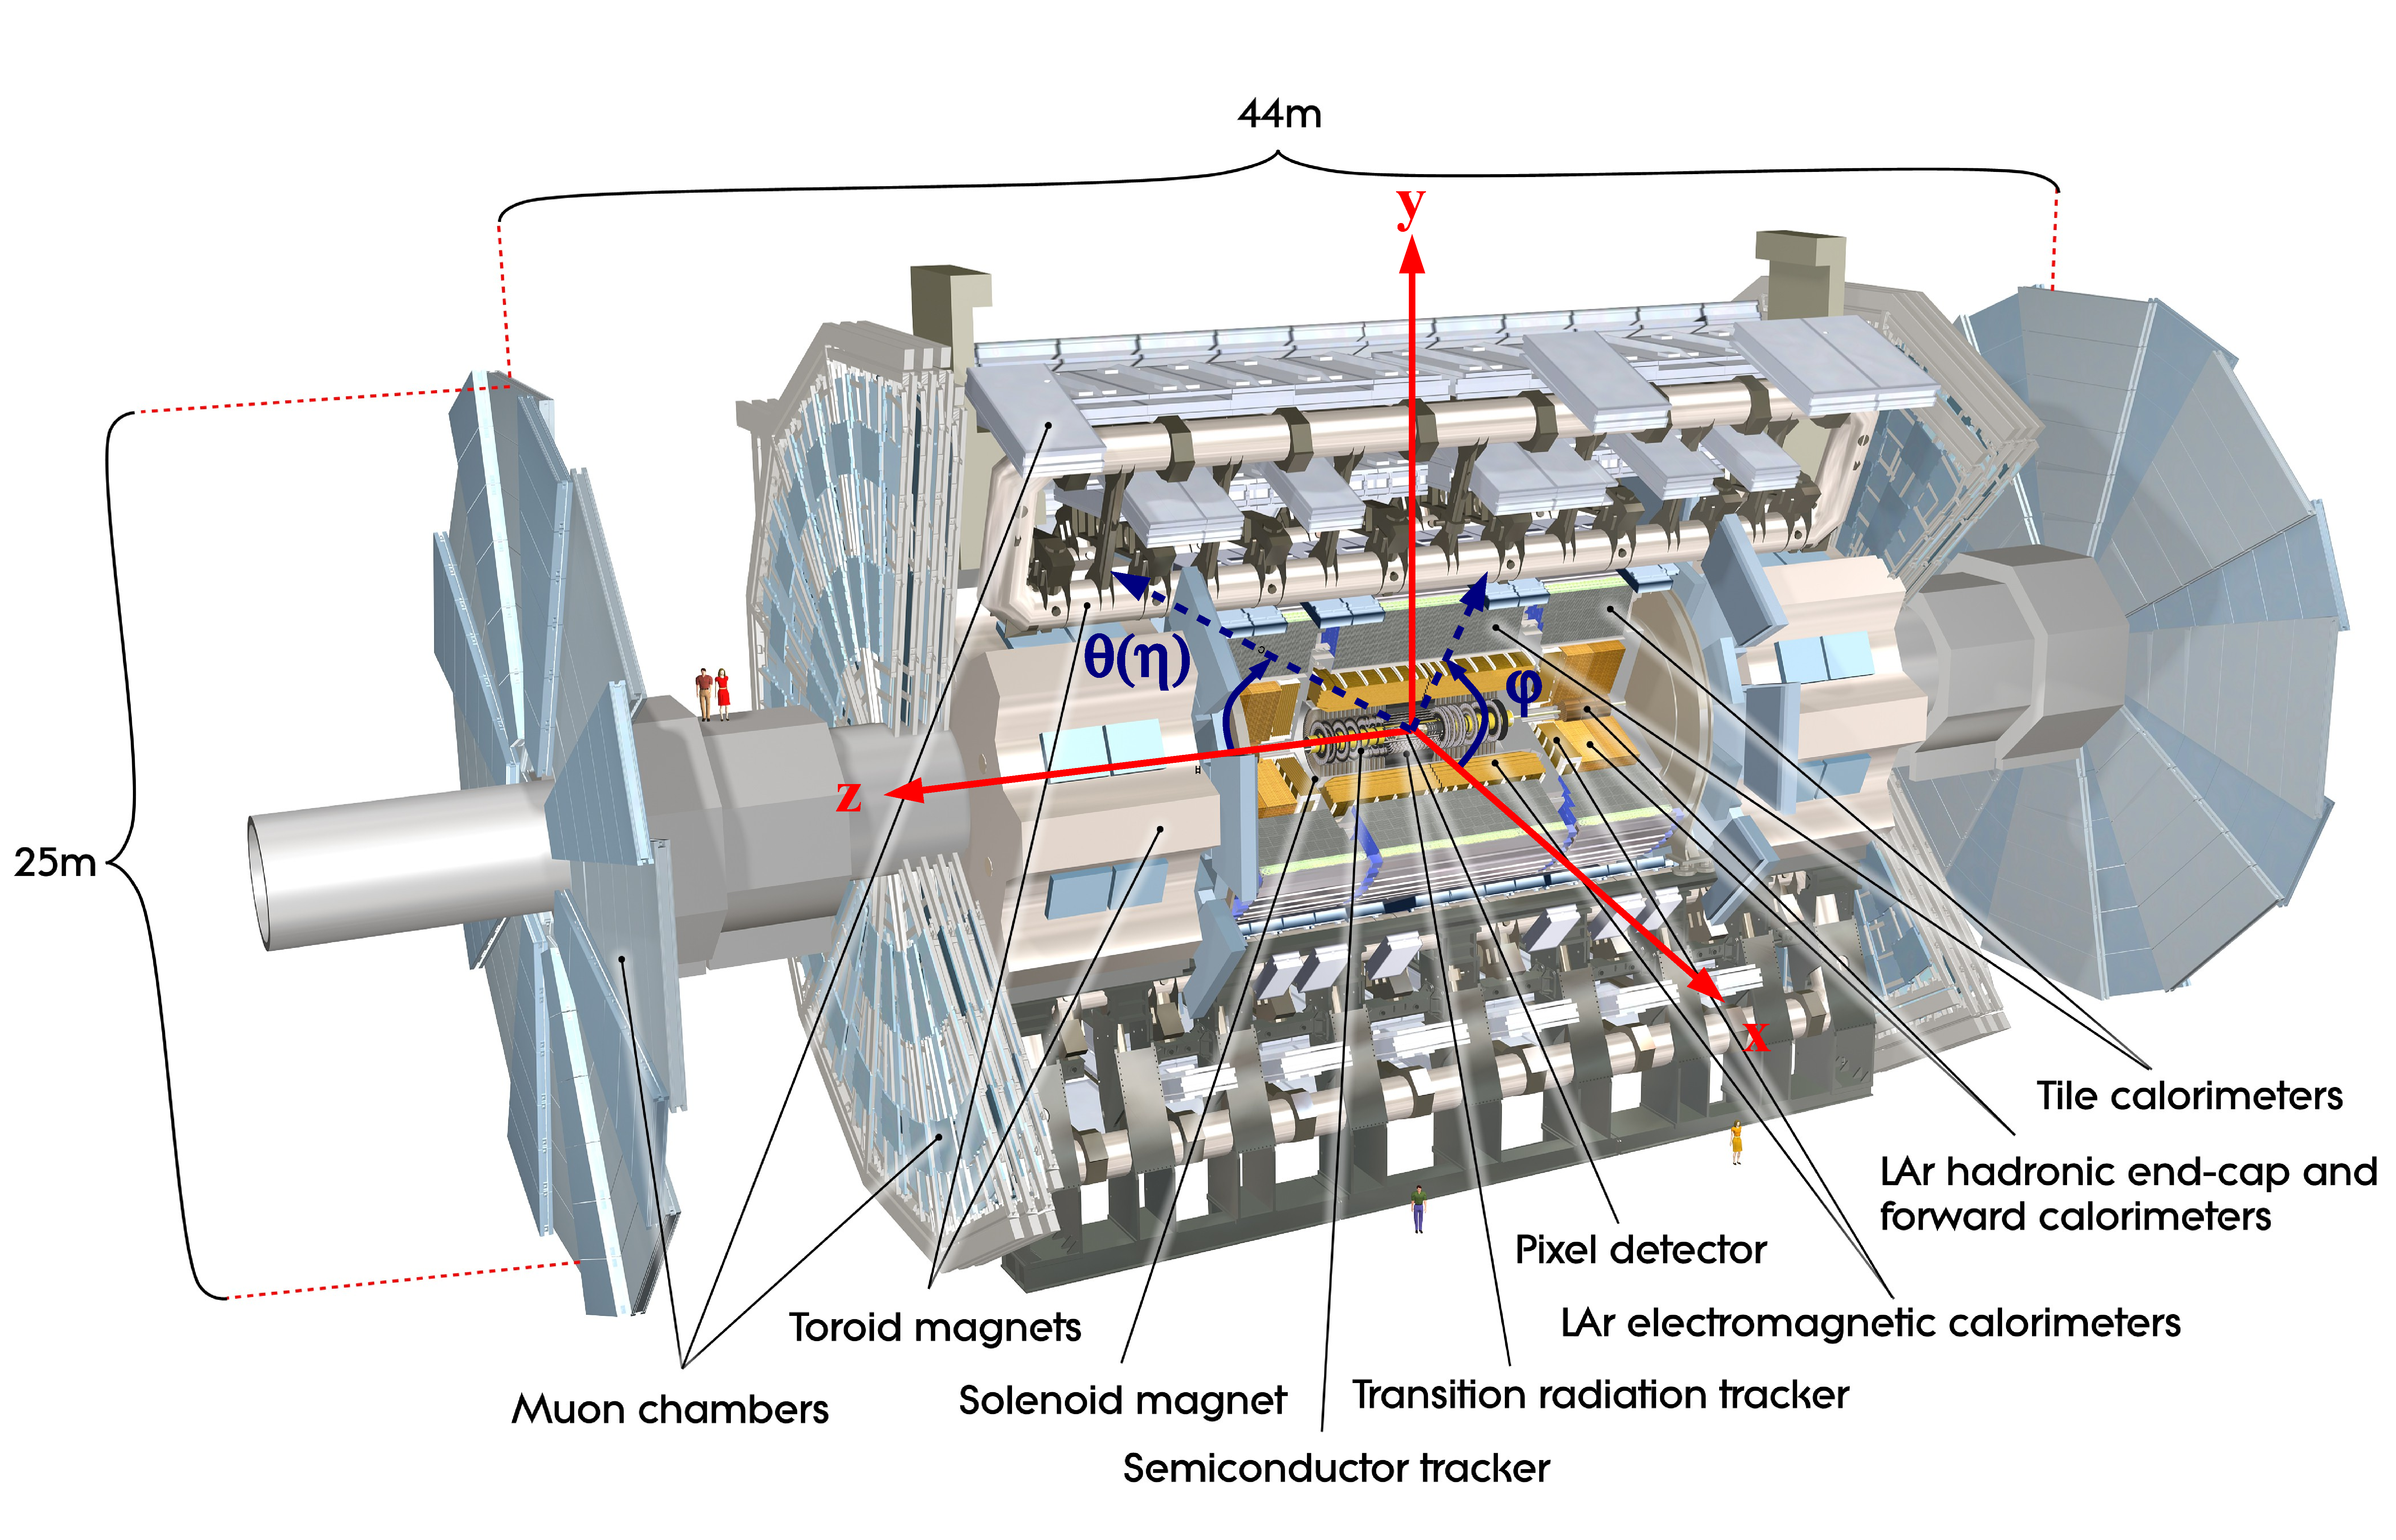
\includegraphics[width=1.1\textwidth]{figures/Detector/atlas_coordinates.png}
\captionsetup{width=0.85\textwidth} \caption{\small View of the ATLAS detector along with the coordinate system.}
\label{sec:det:fig:ATLAScoordinates}
\efig

\subsection{Coordinate system}
The ATLAS coordinate system is right-handed in which $x$-axis points to LHC's center, the $z$-axis follows the beam direction and the $y$-axis points upwards away from the centre of the Earth. The origin of the coordinate system is defined by the nominal interaction point of the beams. The region delimited by positive values of the $z$ coordinate, is referred to as ``A side'', while the region with negative values is referred to as ``C side''. At hadron colliders spherical coordinates are commonly used. The azimuthal angle $\phi$ is measured around the beam axis, ranging between $-\pi$ and $+\pi$ with respect to the $x$-axis. The polar angle $\theta$ is measured with respect to the $z$-axis and ranges between 0 and $\pi$. Since the momentum of the colliding partons along the $z$-axis is unknown, it is useful to define the transverse component of variables of interest, like energy and momentum, defined as the projection on the $xy$ plane, which are boost-invariant along the $z$-axis:
\be
\pt = \sqrt{p_{x}^{2}+p_{y}^{2}}=|\vec p|\sin\theta, \,  E_{T} = E\sin\theta.
\label{sec:det:eq:ptdefinition}
\ee

\noindent Another angular quantity, used at hadron colliders to describe the polar distribution and preferred\footnote{The advantage over $\theta$ is that rapidity differences $\Delta y$ are boost-invariant along the $z$-axis.} to the simple polar angle $\theta$ is the rapidity $y$:

\be
y = \frac{1}{2}\ln\left(\frac{E+p_{\rm z}}{E-p_{\rm z}}\right),
\label{sec:det:eq:rapidity}
\ee

\noindent which, for vanishing particle mass, is equal to the pseudorapidity $\eta$:

\be
\eta = -\ln\left(\tan\frac{\theta}{2}\right).
\label{sec:det:eq:pseudorapidity}
\ee

\noindent The angular separation in the $\eta$-$\phi$ plane between particles is defined as:

\be
\Delta R = \sqrt{(\Delta \eta)^{2}+(\Delta \phi)^{2}}.
\label{sec:det:eq:deltaRdefinition}
\ee



\subsection{Magnet system}
The magnet system \cite{ATLASTDR1} represents a particular characteristic of the ATLAS experiment that has a peculiar design compared to other high-energy physics experiments. It is composed of four large superconducting magnets, cooled with liquid helium at 4.5 K, designed to provide a field mostly orthogonal to the particle trajectory. It consists of a central solenoid and three open-air toroids, as shown in figure \ref{sec:det:fig:ATLASmagnets}. This hybrid solution has the advantage of extending the pseudorapidity coverage ($|\eta|<3$), and having no magnetic field inside the calorimeters in order not to degrade their performances. Furthermore, the open-air design for the toroids reduces the impact of multiple scattering on the momentum resolution and improves the muon reconstruction without relying on the Inner Detector.\par
\bfig[htb!]
\centering
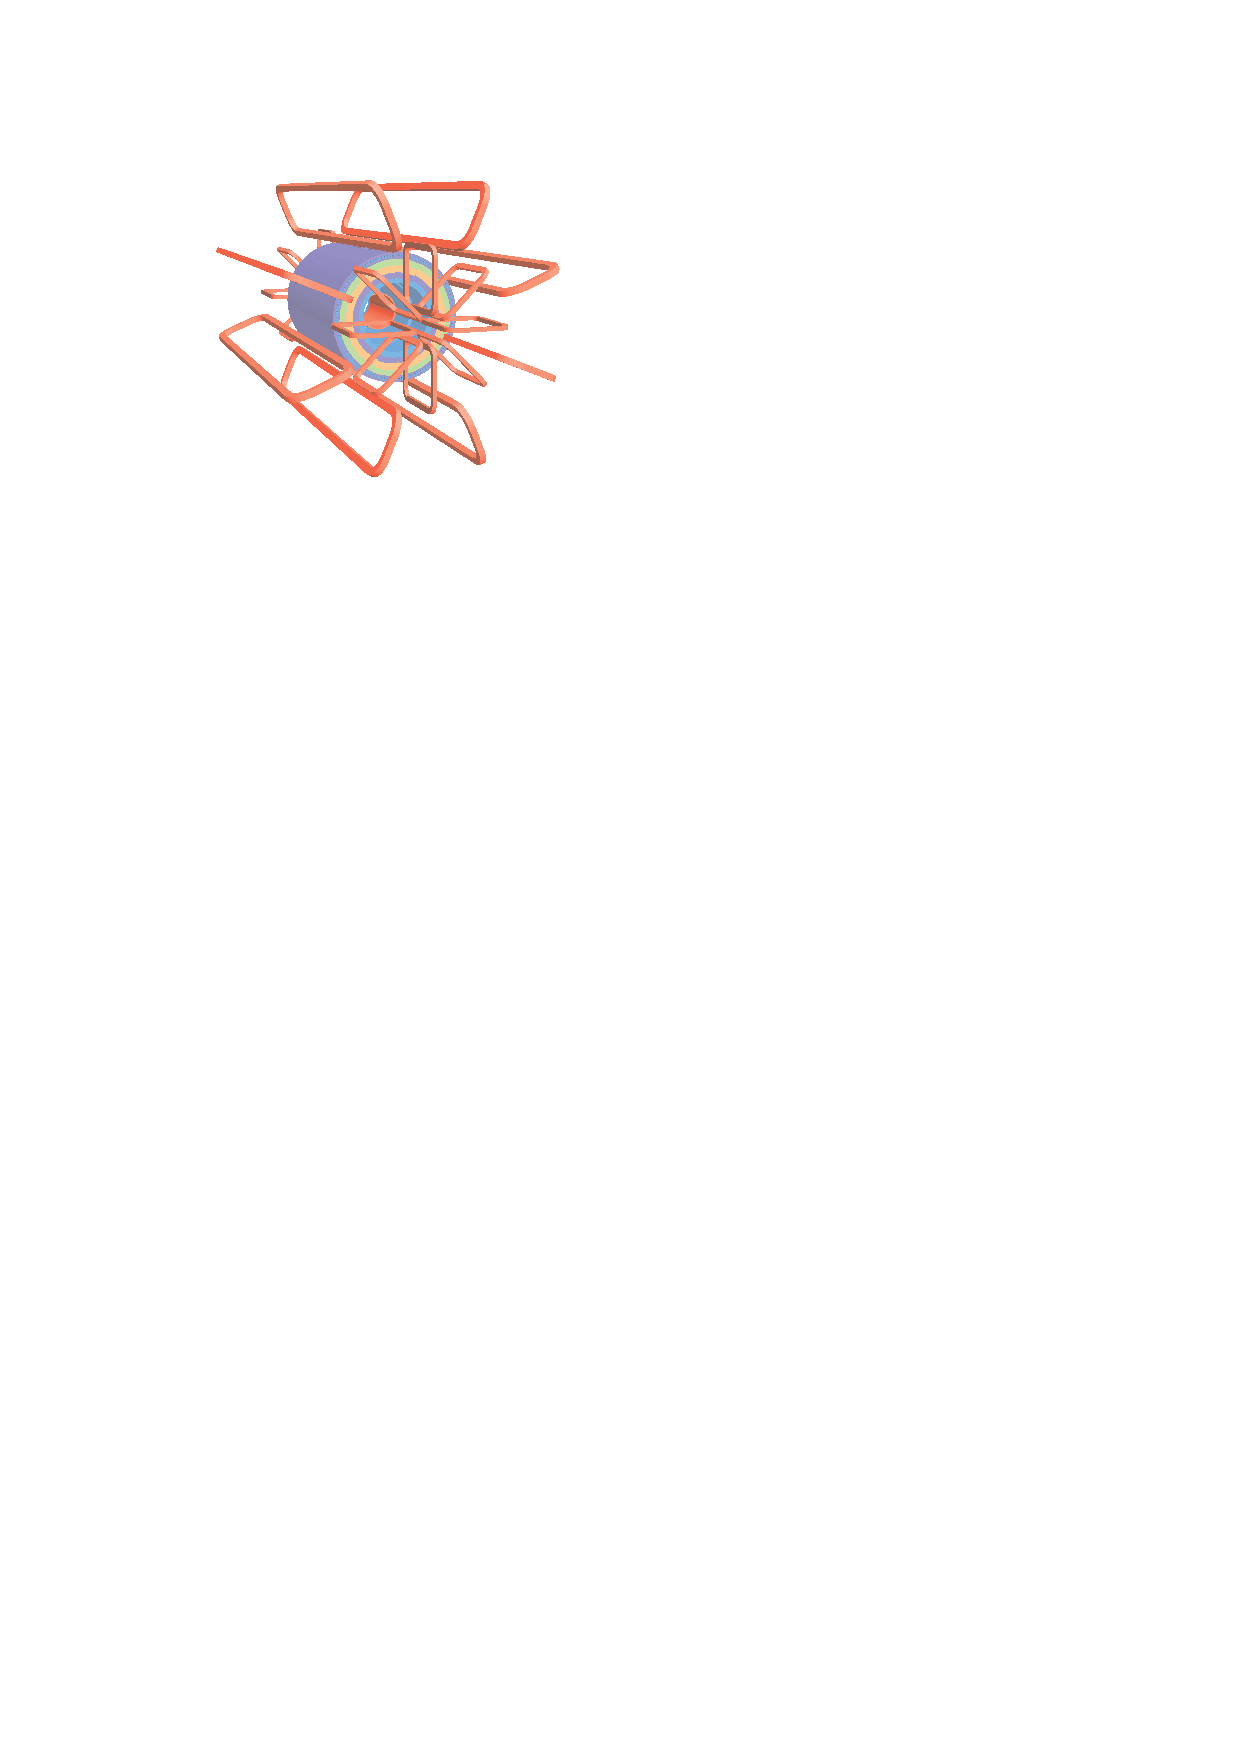
\includegraphics[width=0.5\textwidth]{figures/Detector/magnets.png}
\captionsetup{width=0.85\textwidth} \caption{\small The ATLAS magnet system. The eight coils of the barrel and end-cap toroids are visible. The solenoid is inside the calorimeter and it is shown as four layers with different magnetic properties.}
\label{sec:det:fig:ATLASmagnets}
\efig
The central solenoid (CS) provides a magnetic field to the Inner Detector parallel to the beam axis bending particles in the $\phi$ direction. The CS is 5.3 m long and it has a radius of 2.5 m.  The coil of the CS was designed to be the thinnest possible to limit the amount of material in front of the calorimeters, but still thick enough to ensure safety and reliability during operation. Also to minimise the amount of material in front of the calorimeter, one cooling cryostat is shared between the CS and the Liquid Argon Calorimeter. The magnetic field is 2 T with a peak of 2.6 T on the superconductor. As the distance from the interaction point increases in the $z$ direction, the field strength decreases as result of the finite size of the solenoid.\par
The toroidal system generates the field necessary to bend particles in the muon spectrometer. The system is composed by two End-Cap Toroids (ECT) at the extremities of the detector and a Barrel Toroid (BT) centrally located around the calorimeters. The ECT are 5 m long and have an external diameter of 10.7 m, while the BT is 26 m long with a diameter of 20 m. Each toroid is composed of eight rectangular coils arranged in the radial direction from the beam axis. The ECT are rotated by $22.5^{\circ}$ with respect to the BT in order to generate a radial overlap for a higher magnetic field uniformity and to optimise the bending power in the transition regions. Each coil of the BT has its own cryostat, while for the end-cap toroids all the coils are in the same cryostat that is shared with the forward calorimeter. The magnetic fields generated by the BT and ECT are 3.9 T and 4.1 T respectively. 


\subsection{Inner detector}

The ATLAS Inner Detector (ID) \cite{ATLASTDR1} is designed to provide efficient pattern recognition and good momentum resolution for charged particles in the range $|\eta|<2.5$ from $\pt$ as low as 0.4 $\gev$ up to a few $\tev$. At the same time, its capability of precisely reconstructing primary and secondary vertices and measuring the track parameters is of primary importance for identifying the decays of short-lived particles. A precise measurement of the particle curvature in the solenoidal magnetic field requires a good spatial resolution. In presence of a high density of particles emerging from the interaction point, this can be achieved only with high granularity. The chosen configuration results from a compromise between high performance, economical budget and amount of material used in the tracker. A large amount of material can in fact degrade the intrinsic momentum resolution due to multiple scattering, as well as the performance of the calorimeter. The overall thickness of the ID is about 0.4 radiation lengths ($X_{0}$) and increases up to 1.5 $X_{0}$ in the forward region due to the presence of services (e.g. cables for the electronic boards and the cooling system). The structure of the ID is shown is figure \ref{sec:det:fig:ATLASID}.
 \bfig[tb!]
\centering
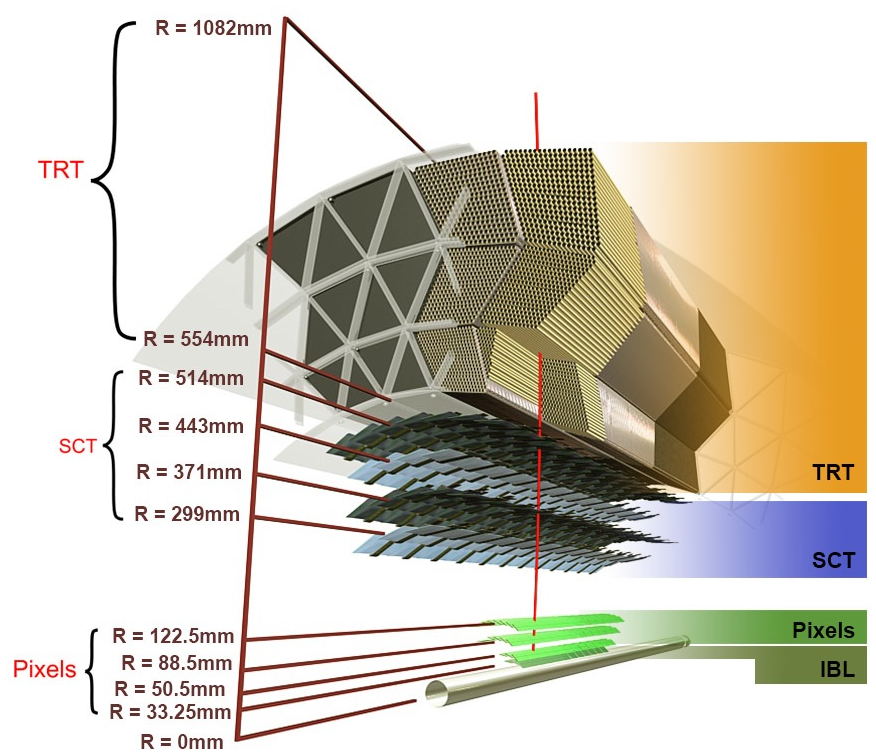
\includegraphics[width=0.7\textwidth]{figures/Detector/fig_01.png}
\captionsetup{width=0.85\textwidth} \caption{\small Representation of the structure of the Inner Detector and its three subdetectors.}
\label{sec:det:fig:ATLASID}
\efig
It combines three different technologies reflecting the different track densities that can be found when increasing the distance from the interaction point. High-resolution detectors are located in the innermost region using semiconductor technology. At larger distance from the interaction point, a detector with lower intrinsic resolution, a transition radiation detector based on drift tubes, allows to collect a larger number of measurements working in a continuous tracking mode.
The three components are:
\bi
\ib Pixel Detector,
\ib SemiConductor Tracker (SCT), and
\ib Transition Radiation Tracker (TRT).
\ei
 
In the barrel the layers of each subdetector are composed of concentric cylinders oriented in the direction of the beam axis while in the forward region are composed of disks/wheels arranged orthogonally to the beam direction. The ID is 7 m long and it has an external radius of 1.15 m, fully contained in the CS. The relative precision of the three subdetectors is comparable so that no single measurements dominates the momentum resolution. This redundancy also guarantees high efficiency even in case a part of one of the subdetectors is malfunctioning. Combining the information from the three subdetectors, the ID reaches a designed resolution of the track momentum of:

\be
\frac{\sigma_{\pt}}{\pt} = 0.05 \% \times \pt(\gev) \oplus 0.1 \%.
\label{sec:det:eq:IDresolution}
\ee



\subsubsection{Pixel detector}

The silicon pixel technology is the only solution that guarantees good pattern recognition performance in a very dense track environment such as the one close to the LHC interaction point. The ATLAS Pixel detector has been designed to provide at least four precise hits for the track reconstruction in the proximity of the interaction point;
 the precise reconstruction of the primary vertex makes use as well of those hits. The pixel detector with its design and location is also important for measurement of the track impact parameter, which is defined as the minimum distance of the track to the primary vertex. This is one of the main quantities used in the identification of $b$/$c$-hadrons and $\tau$-leptons. The resolution on the track impact parameter is completely dominated by the performance of the pixel detector.\par  The detector is organised in a barrel and two end-caps. The barrel is composed of four cylinders: the layer closest to the beam pipe is 62 cm long and has a radius of 3.325 cm (Insertable B-Layer or IBL) \cite{IBLTDR}, installed during the LS1, and the three outer cylinders are 80 cm long and have radii of 5.05 cm (B-Layer), 8.85 cm (Layer 1) and 12.25 cm (Layer 2). Each end-cap contains three disks with a radius of 34 cm placed at distances of $|z|$ = 49.5, 58.0 and 65.0 cm from the centre of the detector. To obtain high granularity the silicon chips are segmented in a matrix of pixels allowing simultaneous measurements of the two spatial coordinates. The dimensions of a single pixel are $50\times250$ $\mu $m$^{2}$ and $50\times400$ $\mu $m$^{2}$ respectively for the IBL and the other layers. The shortest dimension of the sensor is aligned in the direction of the bending plane of the particle in order to achieve the best performance. The average position resolution is equal to 10 $\mu$m in the direction of the short pixel pitch and 65 $\mu$m (115 $\mu$m) in the direction of the long pixel pitch for the IBL (three outer layers). The basic unit of the detector is the module, which contains the silicon sensor and the required electronics. The matrix in each module has $80\time336$ pixels and $144\times328$ pixels respectively in the IBL and the other layers. In total $\sim2500$ modules were assembled in the barrel and endcap for a total of 92 million channels. The pixel detector needs high thermal stability to keep good performance and a low temperature to minimise radiation damage. The IBL temperature during 2015 and 2016 was kept between $-15\,^{\circ}\mathrm{C}$ and $5\,^{\circ}\mathrm{C}$. The other layers are kept at temperature between $-10\,^{\circ}\mathrm{C}$ and $-15\,^{\circ}\mathrm{C}$.

\subsubsection{Semiconductor tracker}

The SCT has been designed to provide at least eight precise points per track. Thanks to its high granularity, it contributes to the track reconstruction and momentum measurement. The detector is organised in a barrel with four cylinders and two end-caps with nine disks. The cylinders have a structure in carbon fibre with radii of 30.0, 37.3, 44.7 and 52.0 cm, on which several longitudinal staves are mounted and equipped with the semiconductor modules. In the end-caps the disks have the modules arranged in the radial direction. The basic unit of the detector is the module and contains two single-sided silicon microstrip sensors mounted back-to-back. Each sensor has an active area of $6.36\times6.40$ cm$^{2}$ and contains 768 microstrips with 80 $\mu$m width. In the barrel the $R-\phi$ coordinate of the hit is determined by the strip position, while a precise measurement of the $z$ coordinate is obtained exploiting the stereoscopic effect: the back-to-back sensors are mounted with a 40 mrad ``tilt'' angle, so the crossing point of the strips on both sensors on each module is used to determine the space-point position. In the end-cap, the $\phi$ coordinate of the track is determined using the strip position and the $R$-coordinate with the ``stereo'' effect. The spatial resolution achieved is 17 $\mu$m in the direction of the strip pitch, and 580 $\mu$m in the direction determined by the strip crossing. For the same reasons as in the Pixel Detector, the SCT is kept at a temperature between $-5\,^{\circ}\mathrm{C}$ and $-15\,^{\circ}\mathrm{C}$.

\subsubsection{Transition radiation tracker}
The TRT, the outermost part of the three tracking subsystems of the ID, is a straw-tube tracker particularly well suited to LHC conditions due to its resistance to radiation. The barrel region contains 52544 straw tubes with a length of 1.5 m arranged parallel to the beam axis. Barrel tubes have the central wires electrically split and read out at both ends of the straw. Each end-cap contains 122880 straw tubes with a length of 0.4 m arranged perpendicularly to the beam axis, and read out at their outer end. Each drift tube has a diameter of 4 mm that is made from wound Kapton and carbon fibre; in the centre of each tube there is a gold-plated tungsten wire of 31 $\mu$m diameter and the tube is filled with a gas mixture. Most of the TRT is filled with a mixture of $70\,\%$ Xe, $27\,\%$ CO$_{2}$, and $3\,\%$ O$_{2}$. Due to large irreparable gas leaks that developed in the gas system, part of the TRT detector is now flushed with a gas mixture composed primarily of much cheaper argon, $80\,\%$ Ar and $20\,\%$ CO$_{2}$ (see figure \ref{sec:det:fig:trfgas}).

\begin{figure}[tb!]
  \begin{subfigure}{0.5\textwidth}
  \centering
  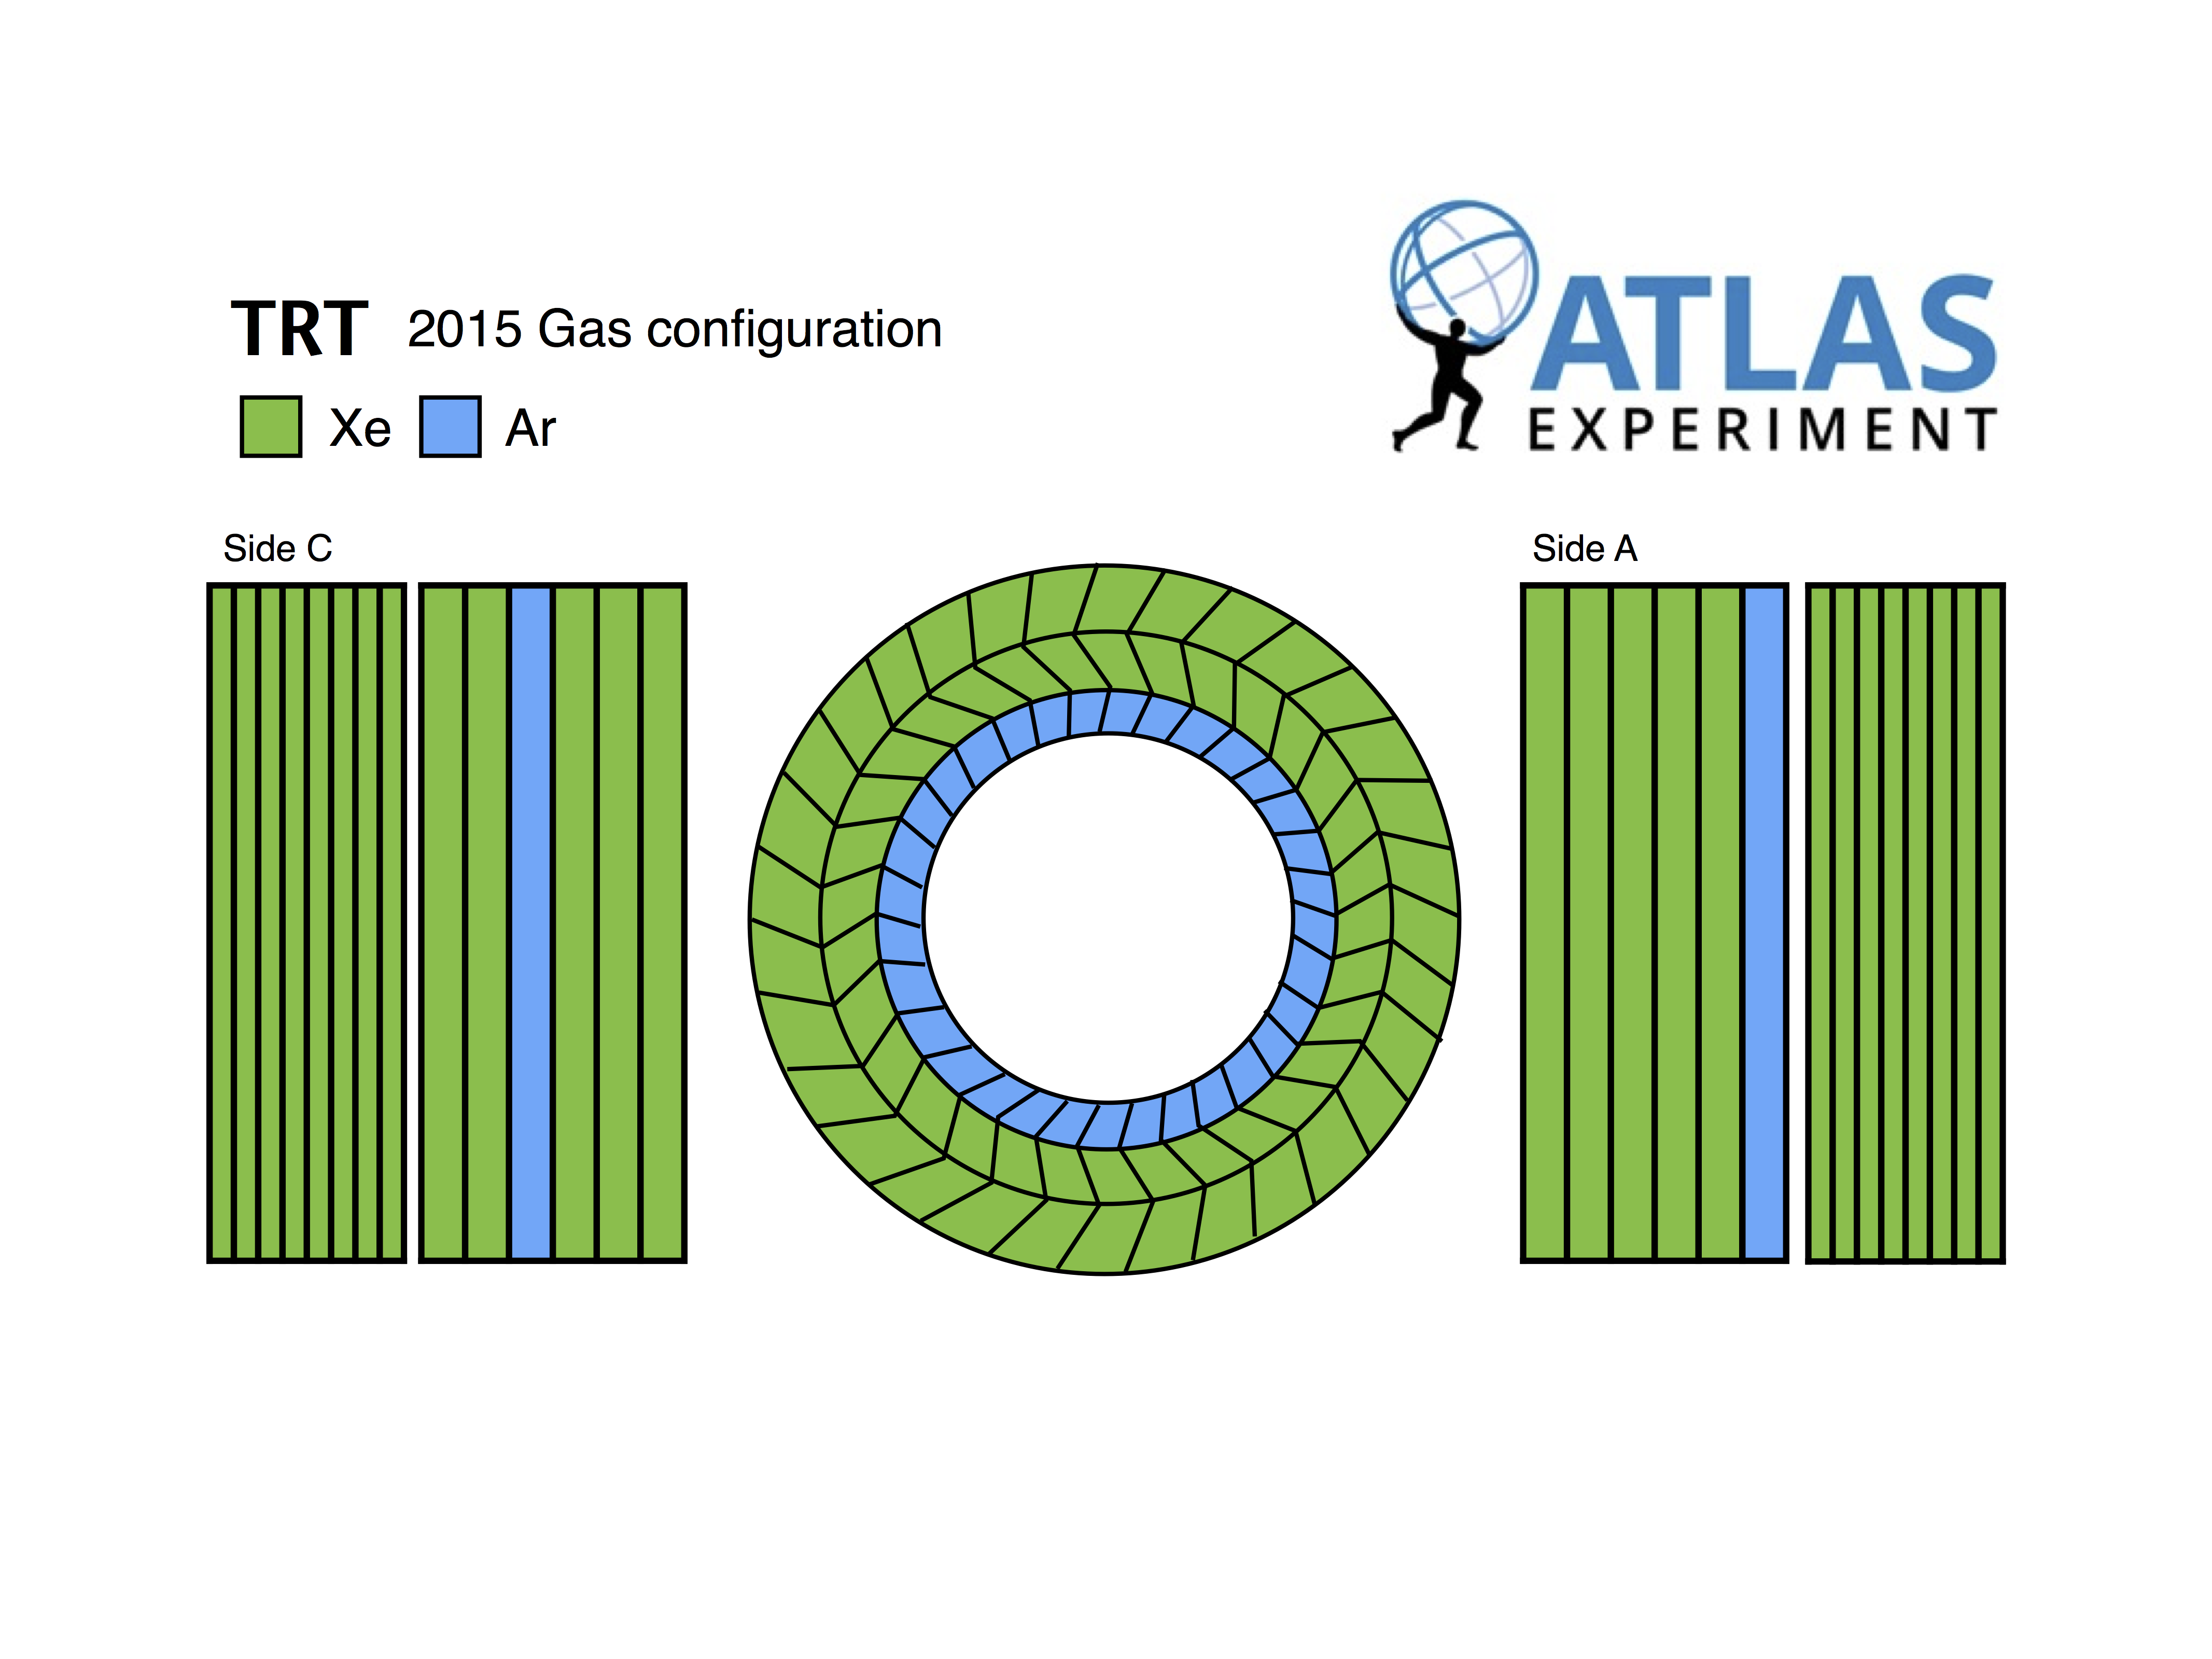
\includegraphics[width=0.9\textwidth]{figures/Detector/trtfig_01.png}
  \caption{}
  \label{chp:det:atlas:trt2015}
\end{subfigure}
\begin{subfigure}{0.5\textwidth}
  \centering
  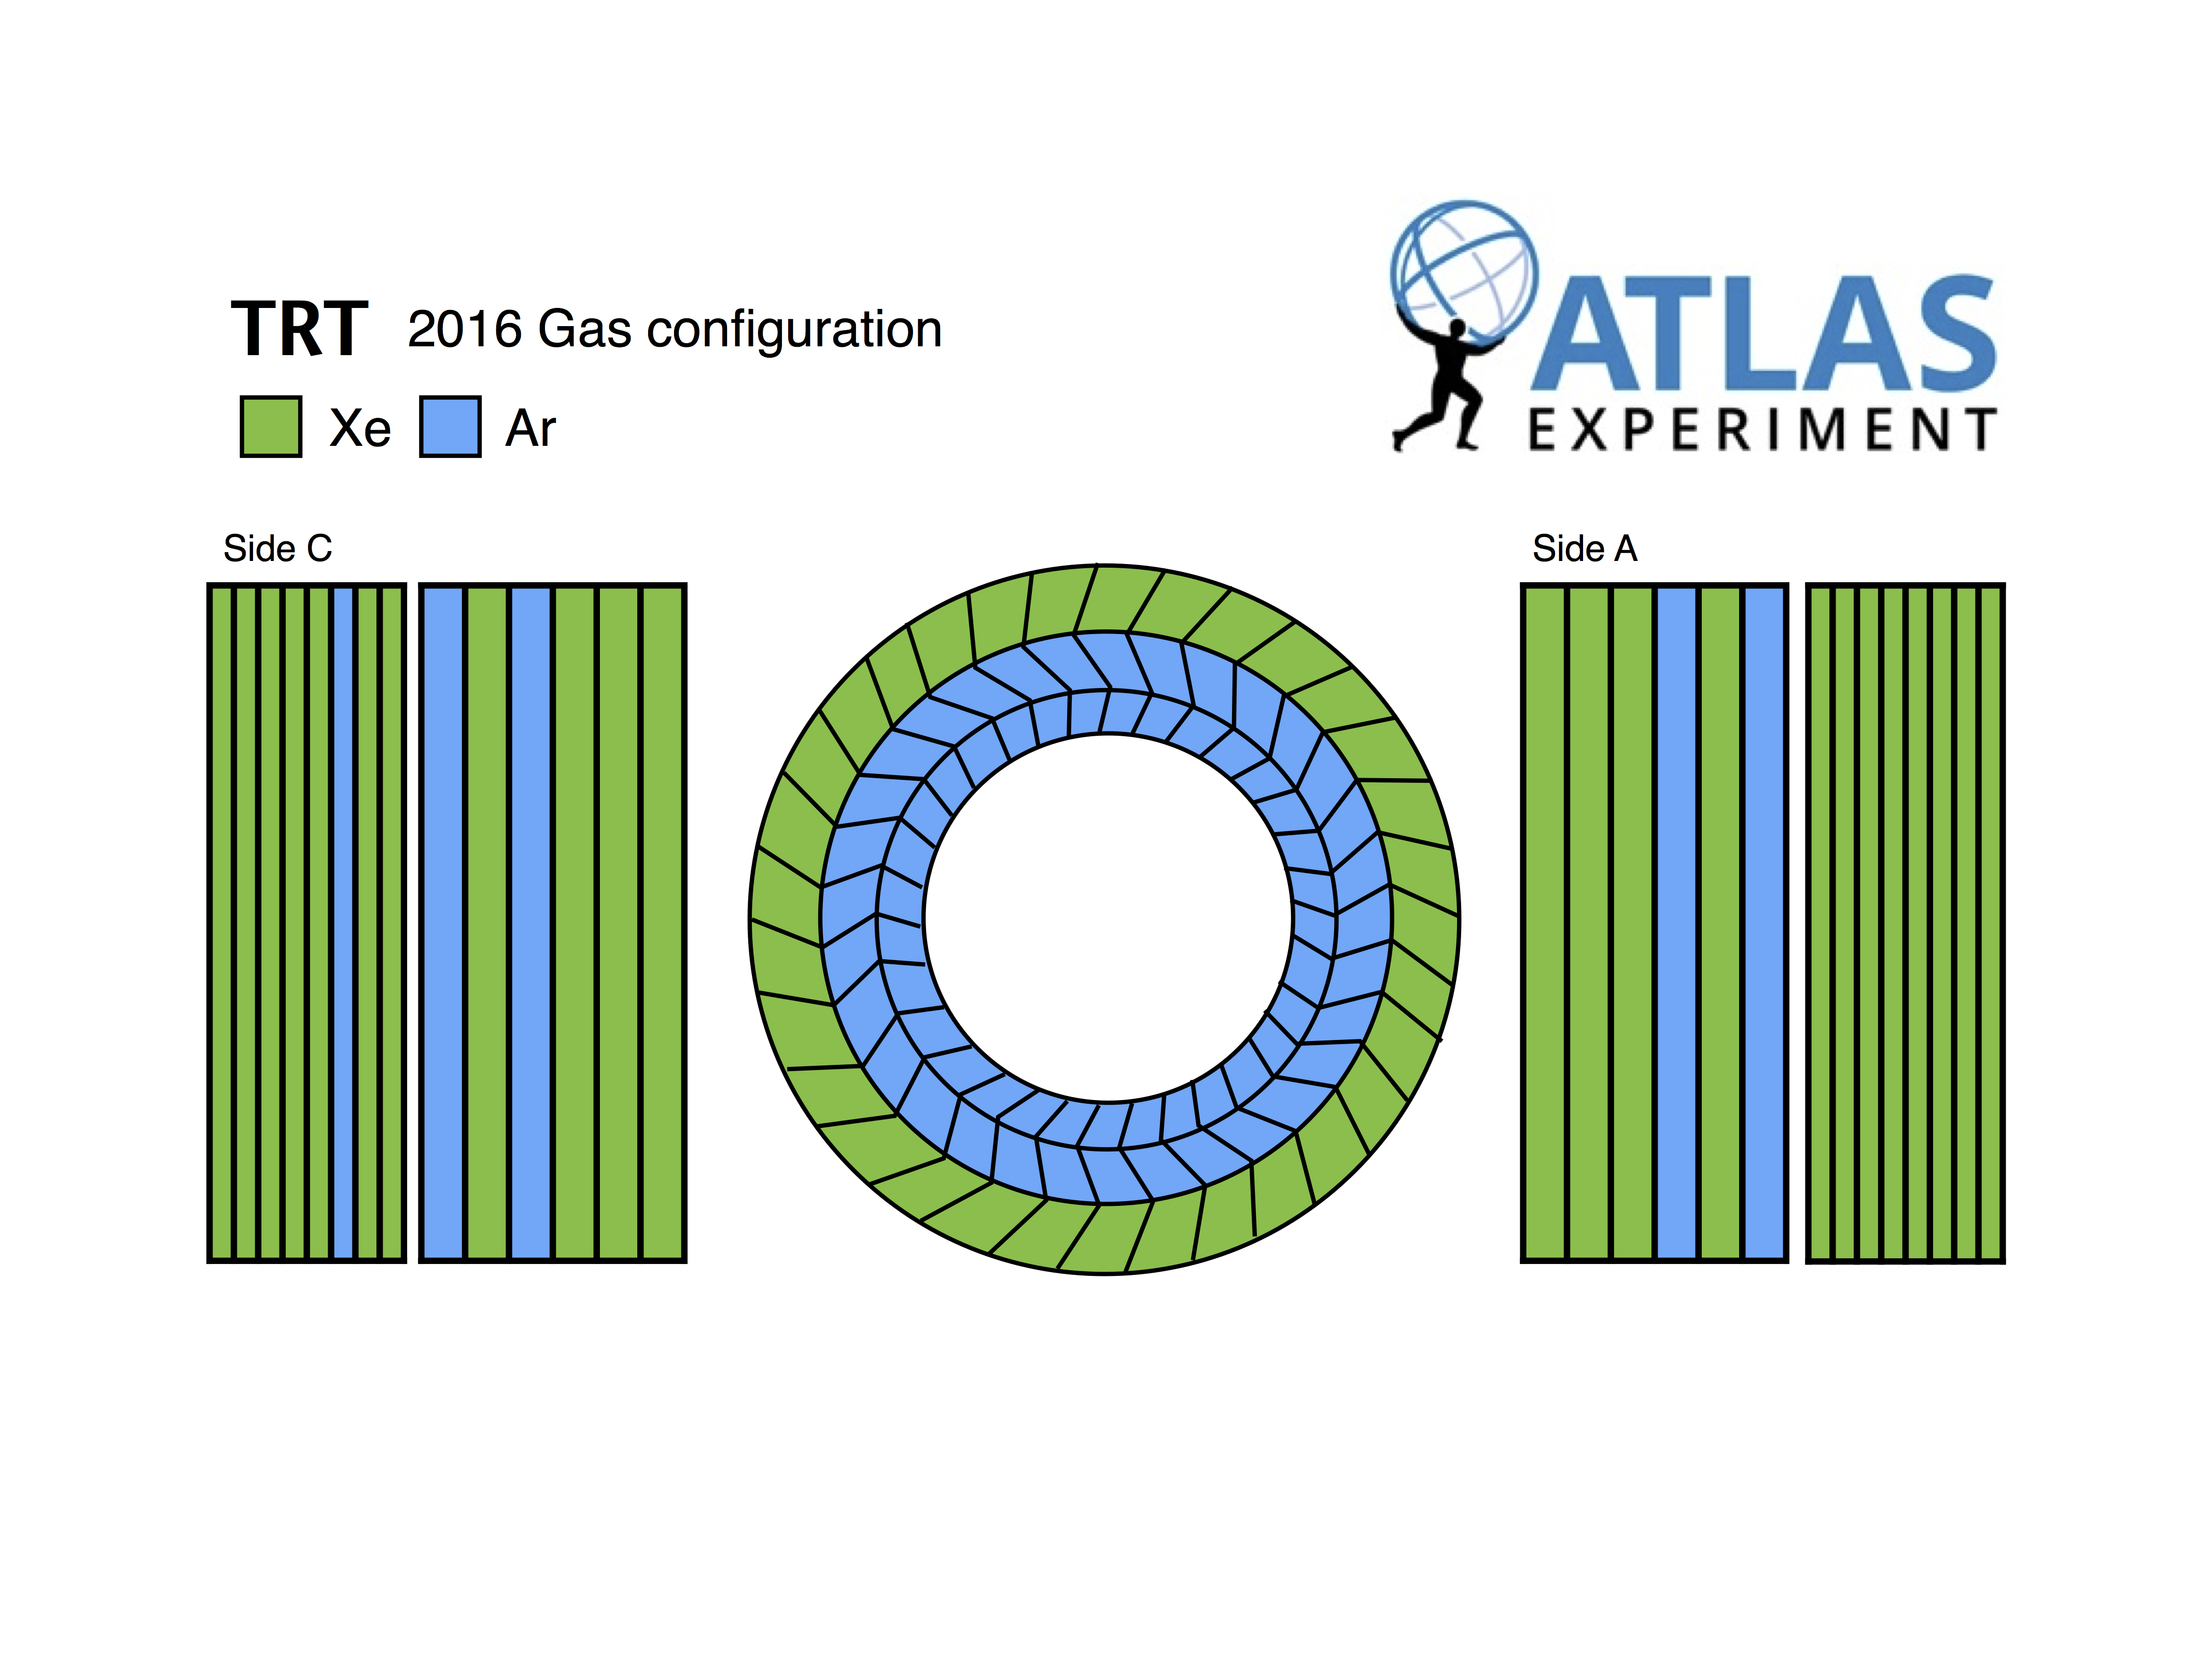
\includegraphics[width=0.9\textwidth]{figures/Detector/trtfig_02.png}
  \caption{}
  \label{chp:det:atlas:trt2016}
\end{subfigure}

\captionsetup{width=0.85\textwidth} \caption{\small TRT gas configuration used in the year (a) 2015 and (b) 2016.}
\label{sec:det:fig:trfgas}
\end{figure}


The spaces between the straws are filled with polymer fibres (barrel) and foils (end-caps) to create transition radiation, which is emitted by highly-relativistic charged particles as they
traverse a material boundary. This effect depends on the Lorentz boost $\gamma$ $(E/m)$ and is strongest for electrons, which means it can be used for particle identification. X-rays coming from the transition radiation process can be absorbed by the noble gas, resulting into additional energy being deposited into the gas. This design  makes the TRT complementary to  the silicon-based tracking devices. Each channel, through the tube drift time measurement, has an intrinsic single-point resolution of $120$ $\mu$m, larger than that of the silicon trackers, but this is compensated by the large number of hits per track (typically more than 30) and the long lever arm.  Furthermore, the high sampling frequency of the wire signals enables the TRT to provide timing information at the nanosecond level.

\subsection{Calorimeters}
The ATLAS calorimeter system \cite{ATLASTDR1} surrounds the ID and it consists of an inner electromagnetic calorimeter and an outer hadronic calorimeter. It was designed to provide full coverage in $\phi$ and to measure a wide range of energy deposits over the entire pseudorapidity coverage of $|\eta|<4.9$ from both neutral and charged particles. The structure of the ATLAS calorimeter is shown in figure \ref{sec:det:fig:ATLASCALO}. In the acceptance region covered by the ID, the granularity of the EM calorimeter is finer in the $\eta$ and $\phi$ directions in order to provide precision measurements of electrons and photons. The rest of the calorimeter system has coarser granularity, yet appropriate for a precise measurement of jet kinematics, and provides sufficient longitudinal containment of the showers  in order to calculate the missing transverse energy.
All of the ATLAS calorimeters are sampling calorimeters; they consist of absorber sheets, which initiate particle showers, alternated with layers of active
medium material to perform energy measurements. When a particle reaches the calorimeter, it produces showers in stages, loosing more and more energy until the shower is completely absorbed. The energy of the initial particle is then obtained by summing up all energy deposits within the active material of the calorimeter. The calorimeter is designed to fully absorb the particle energy to avoid losses caused by escaping particles. It also reduces possible punch-through to the muon chambers by energetic hadrons.

\bfig[t!]
\centering
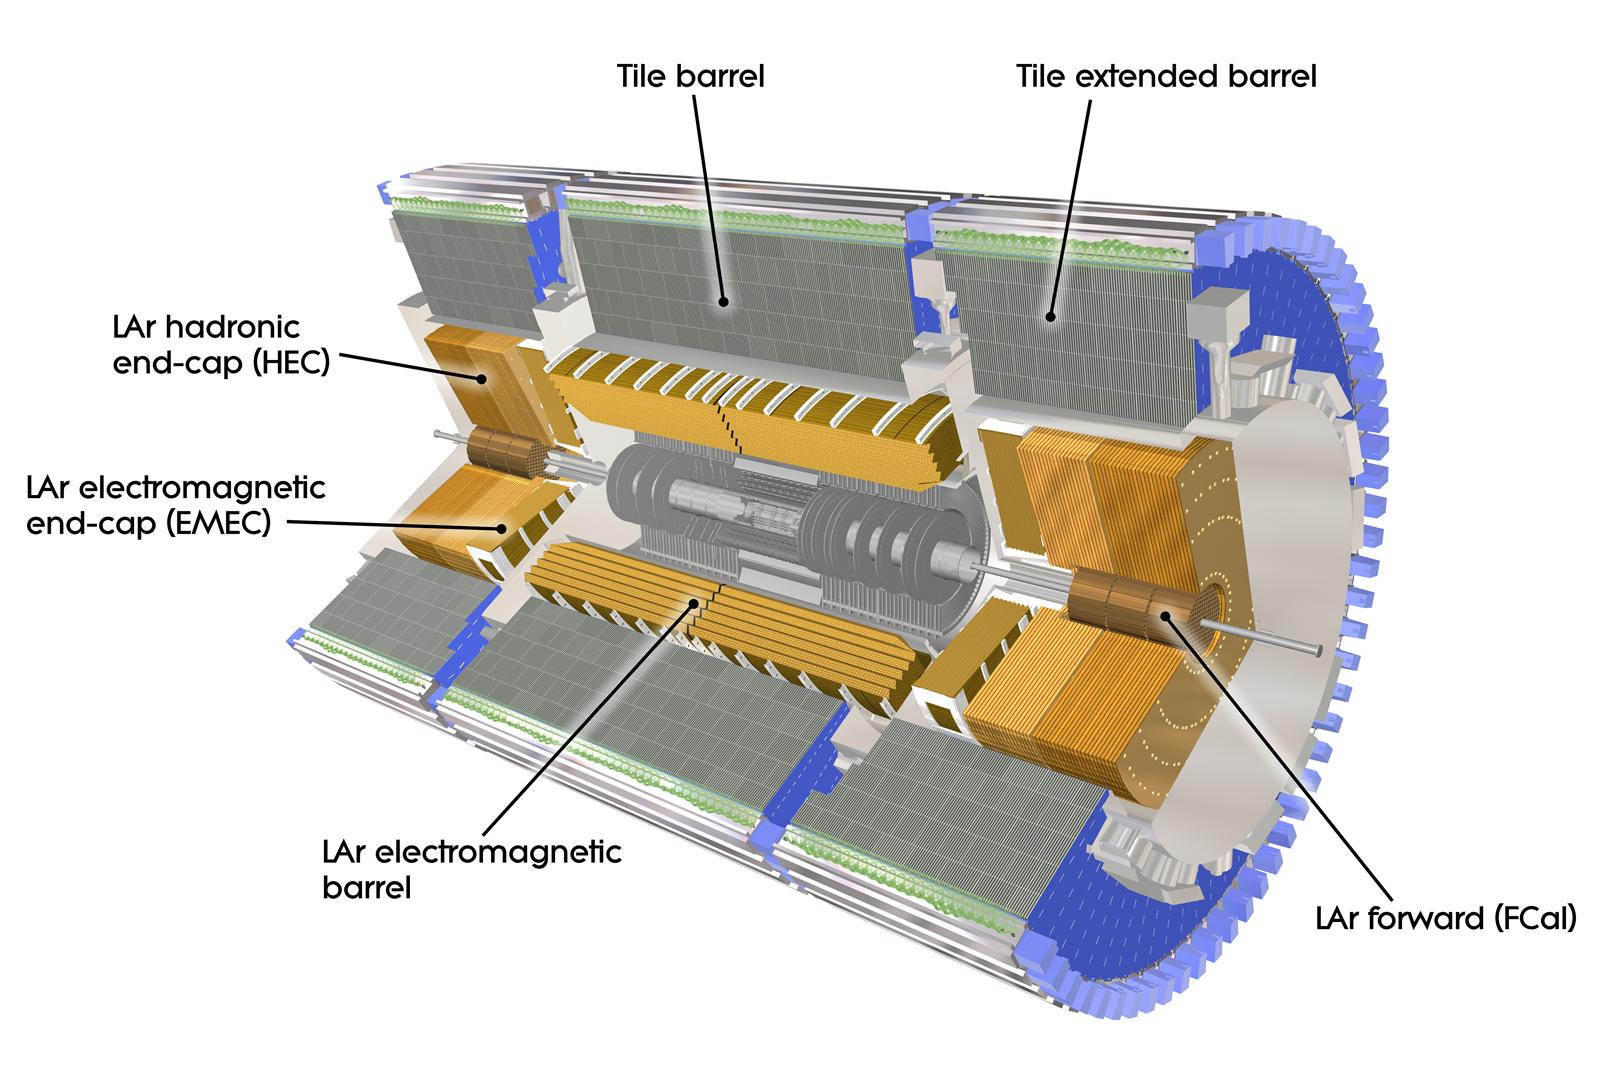
\includegraphics[width=0.8\textwidth]{figures/Detector/calo_all}
\captionsetup{width=0.85\textwidth} \caption{\small Schematic view of the ATLAS calorimeter system.}
\label{sec:det:fig:ATLASCALO}
\efig

\subsubsection{Electromagnetic calorimeter}

The  Electromagnetic CALorimeter (ECAL) is  divided  into  a  barrel  part  ($|\eta|< 1.475$)  and  two  end-caps ($1.375 <|\eta|< 3.2$). The barrel calorimeter consists of two identical half-barrels, separated by a small gap (6 mm) at $z=0$. Each end-cap calorimeter is mechanically divided into two coaxial wheels: an outer wheel covering the region $1.375 <|\eta|< 2.5$, and an inner wheel covering the region $2.5 <|\eta|< 3.2$.
The ECAL uses liquid argon (LAr) as active material with accordion-shaped Kapton electrodes and lead absorber plates over its full coverage. The LAr solution was adopted for its intrinsic linear behaviour, high ionisation yield and stability. The LAr gas is constantly flowing and does not suffer from radiation damage; LAr is therefore preferable in the region close to the interaction point, as well as in the very forward regions. The accordion geometry provides complete $\phi$ symmetry without  azimuthal  cracks.  The  lead  thickness  in  the  absorber  plates  has  been  optimised  as  a function of $\eta$ in terms of EM energy resolution. High voltage is applied between absorber plates to collect ionisation electrons  from the interaction with the LAr as well as to produce signal amplification.
The total thickness of the ECAL is >24~$X_{0}$ in the barrel and >26~$X_{0}$ in the end-caps. This ensures the absorption of electron and photon showers up to few $\tev$ of energy and around 2/3 of typical hadronic showers. Over the region devoted to precision physics ($|\eta|< 2.5$), the ECAL is segmented into three longitudinal sections with different cell structure in the $\eta-\phi$ plane. 
The first layer, which has a constant thickness of $\sim6\,X_{0}$ (upstream material included) as a function of $\eta$, is equipped with narrow readout strips of $\Delta \eta \times \Delta \phi =  0.0031 \times 0.098$.  This  section  acts  as  a  ``preshower''  detector,  enhancing  particle  identification ($\gamma/\pi^{0}, e/\pi$ separation, etc) and providing a precise position measurement in $\eta$. The second layer is  transversally  segmented  into  square  towers  of size $\Delta \eta \times \Delta \phi =  0.025 \times 0.025$  ($\sim 4\times$4 cm$^{2}$ at $\eta=0$). 
The total calorimeter thickness up to the end of the second section is $\sim24$ $X_{0}$, tapered with increasing rapidity (this includes also the upstream material). Combining the information from the first two layers provides a precise measurement of a photon's production vertex. The third layer has a granularity of 0.05 in $\eta$ and a thickness varying between 2 $X_{0}$  and 12 $X_{0}$. For $|\eta|> 2.5$, i.e. for the end-cap inner wheel, the calorimeter is segmented in two longitudinal sections and has a coarser lateral granularity than for the rest of the acceptance. The calorimeter cells point towards the interaction region over the complete eta coverage.  In the region where the amount of material exceeds $\sim2$ $X_{0}$ (as is the case for $|\eta|< 1.8$), a presampler is used to correct for the energy lost by electrons and photons upstream of the calorimeter. The presampler consists of an active LAr layer of thickness 1.1 cm (0.5 cm) in the barrel (end-cap) region. In figure \ref{chp:det:atlas:ATLASECAL} the structure of the ECAL is shown. The total number of channels for the entire ECAL is $\sim$190 000. 
The design energy resolution is:

\be
\frac{\sigma_{E}}{E} = \frac{9\%}{\sqrt{E\,(\gev)}} \oplus 0.3 \%, 
\label{sec:det:eq:ECALresolution}
\ee

\noindent while the angular resolution is $\sigma_\theta \sim 50$ mrad/$\sqrt{E(\gev)}$.


\begin{figure}[t!]
\begin{subfigure}{0.5\textwidth}
  \centering
  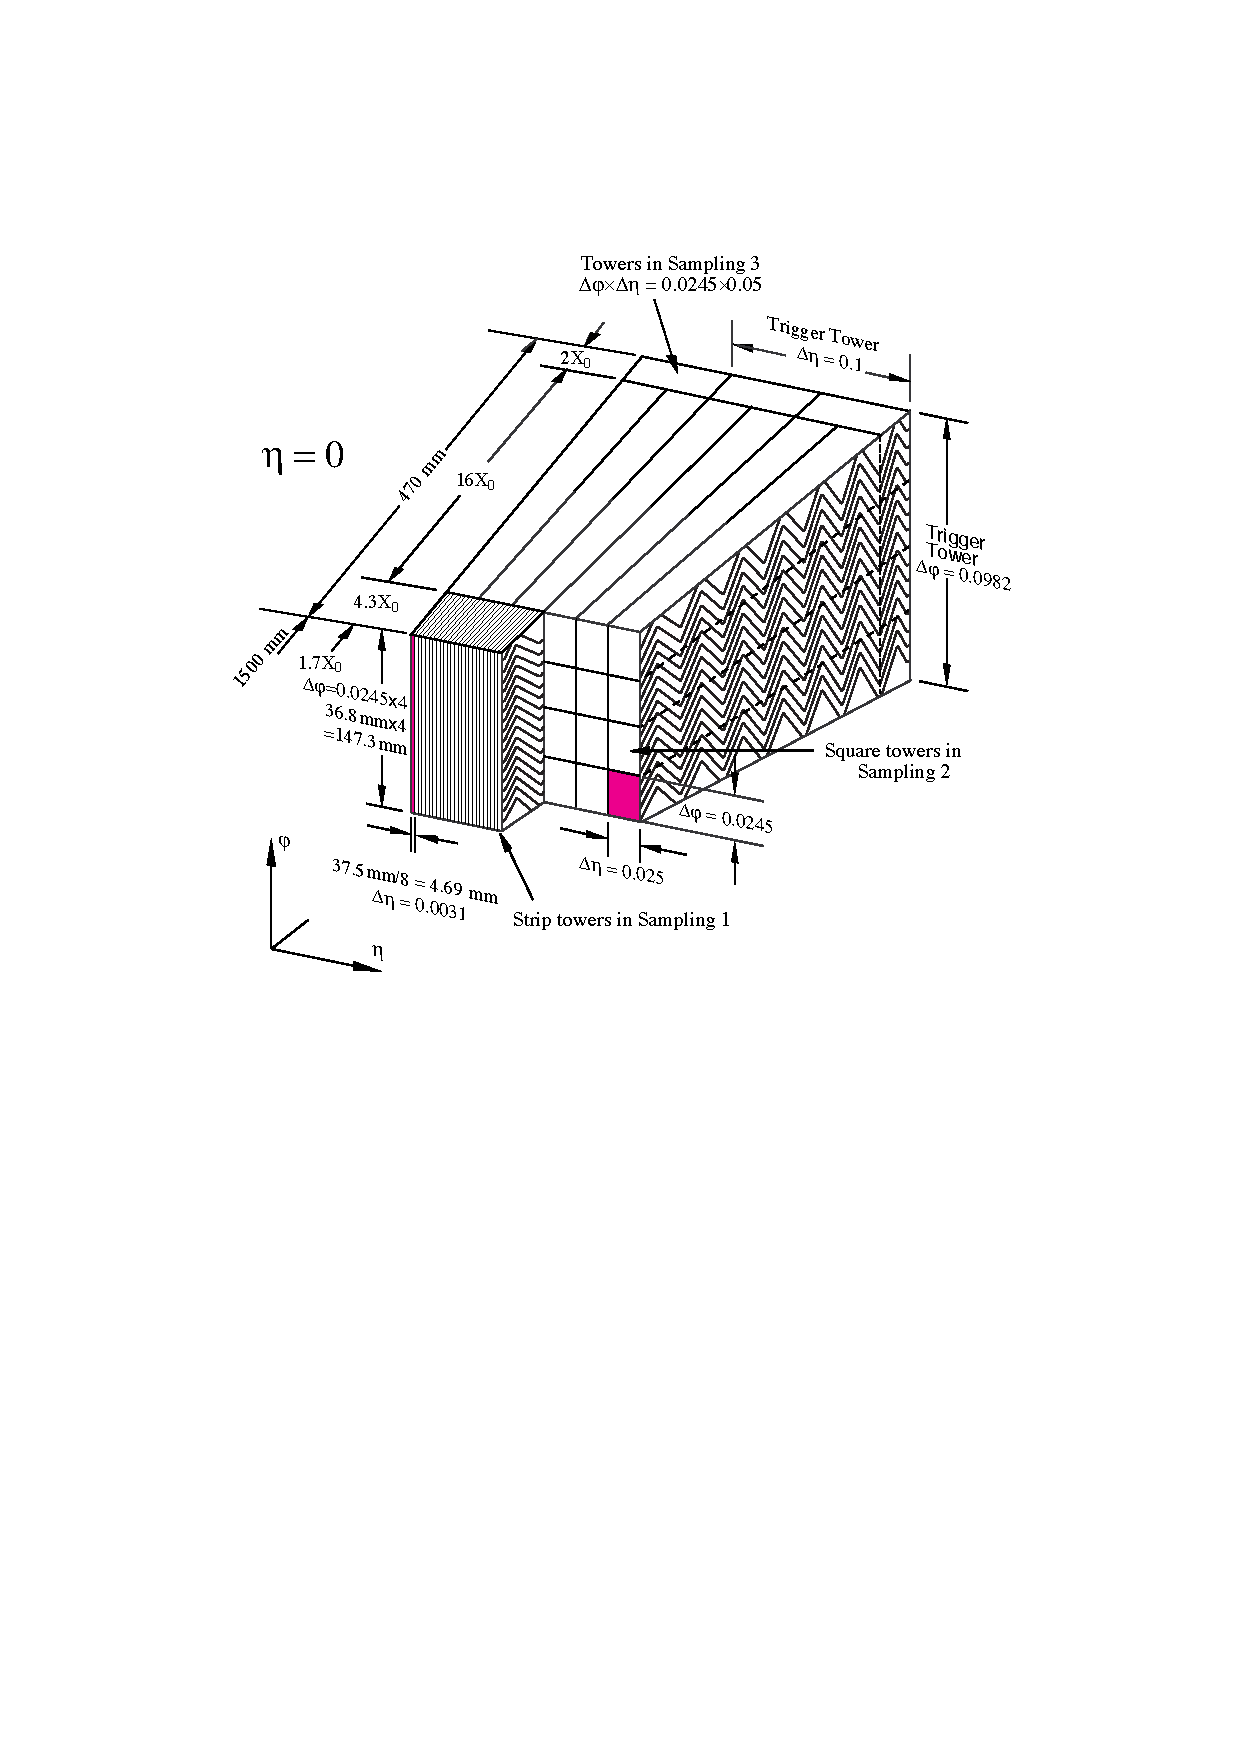
\includegraphics[width=0.9\textwidth]{figures/Detector/larg_module.png}
  \caption{}
  \label{chp:det:atlas:ATLASECAL}
\end{subfigure}
\begin{subfigure}{0.5\textwidth}
  \centering
  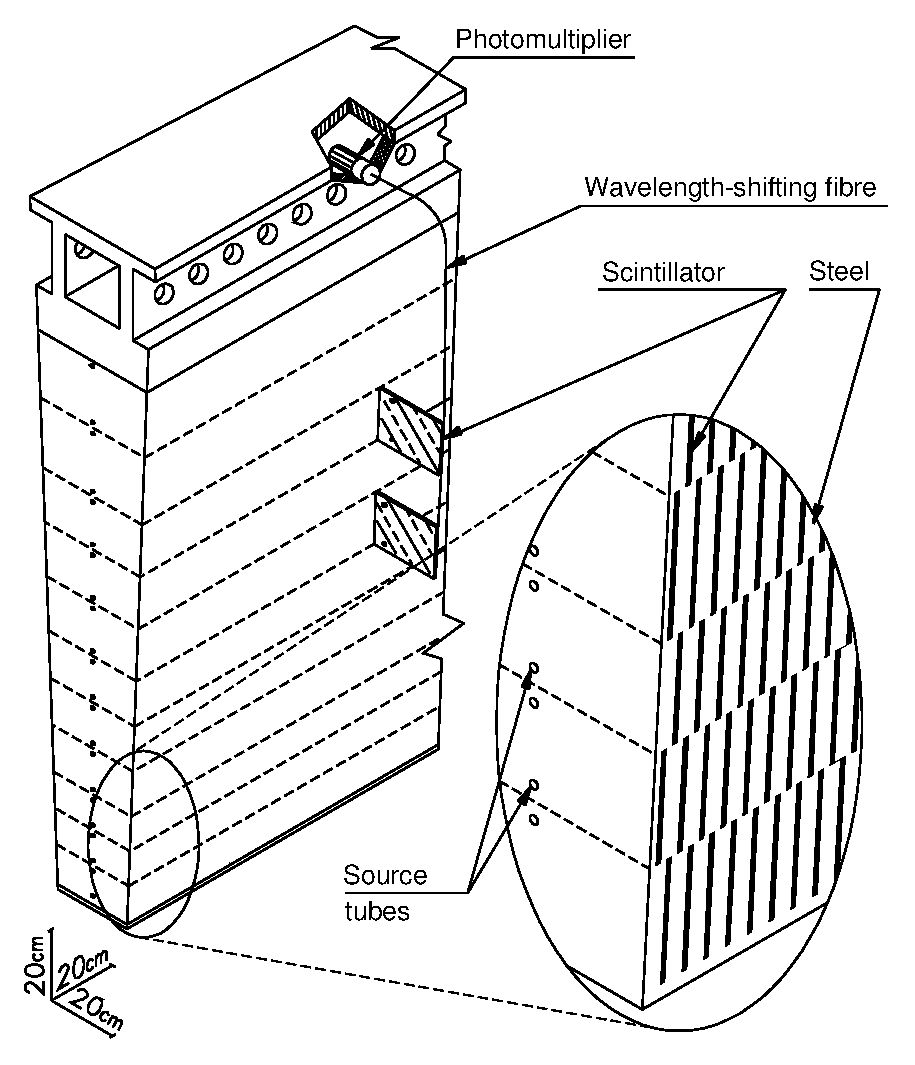
\includegraphics[width=0.8\textwidth]{figures/Detector/TileCal_Module.eps}
  \caption{}
  \label{chp:det:atlas:ATLASTILECAL}
\end{subfigure}

\caption{Schema of different modules of the ATLAS calorimeters: (a) electromagnetic
calorimeter and (b) hadronic calorimeter.}
\label{chp:det:atlas:cal}
\end{figure}



\subsubsection{Hadronic calorimeter}
The ATLAS hadronic calorimeters cover the range $|\eta|< 4.9$ using different techniques best suited for the widely-varying requirements and radiation environment over the large $\eta$ range. An important parameter in the design of the hadronic calorimeter is its thickness: it has to provide good containment for hadronic showers and reduce punch-through into the muon system to a minimum. The total thickness is 11 interaction lengths ($\lambda$) at $\eta = 0$, including about 1.5 $\lambda$ from the outer support, which has been shown both by measurements and simulation to be sufficient to reduce the punch-through well below the irreducible level of prompt or decay muons. Close to 10 $\lambda$ of active calorimeter are adequate to provide good energy resolution for high-energy jets. Together with the large $\eta$ coverage, this also guarantees a good \MET  measurement.
In the central region the Tile calorimeter covers the range $0 < |\eta| < 1.7$ (11.4 m long cylinder with an inner radius 2.28 m and an outer radius of 4.25 m). The Tile calorimeter is composed of one barrel and two extended barrels. It consists of a sampling calorimeter that uses scintillating tiles as the active material and steel as the absorber arranged in three layers. Scintillator tiles, approximately 3 mm in thickness, are arranged radially along the beam pipe with the tile face along the $z$-axis, with steel absorbers sandwiched between the tiles in this orientation. The scintillation light induced in a tile upon the passage of radiation is read out by optical fibres and sent into two separate photomultiplier tubes. Azimuthally, the barrel and extended barrels are divided into 64 modules. In $\eta$, the readout cells, built by grouping fibres into PMTs, are ``pseudo-projective'' towards the interaction region. The resulting granularity is $\Delta \eta \times \Delta \phi =  0.01 \times 0.01$ ($0.2\times0.1$ in the last layer).
The region $1.5< |\eta| < 3.2$ is covered by the Hadronic End-cap Calorimeter (HEC), which uses copper plates as absorbers and LAr as active material for its superior radiation resistance. It  consists of two independent wheels with an outer radius of 2.03 m. Each wheel is built out of 32 identical modules, assembled with fixtures at the periphery, and a central ring. As for the electromagnetic calorimeter, the electric signal produced in the LAr is collected by cathodes on the plates. 
Finally, in the most forward part ($3.1< |\eta| <4.9$) a Forward Calorimeter (FCAL) is present. It is assembled with tungsten rod absorbers embedded in a copper matrix. Between the two, a thin gap filled with LAr provides the active material. The radial depth of the hadronic calorimeter is approximately 7.4 $\lambda$ with minimal variation across the $\eta$ range.  The resolution achieved in this configuration is:
\be
\frac{\sigma_{E}}{E} = \frac{50\%}{\sqrt{E\,\gev}} \oplus 3 \% \text{ for Tile and HEC, and}
\label{sec:det:eq:TILEresolution}
\ee
\be
\frac{\sigma_{E}}{E} = \frac{100\%}{\sqrt{E\,\gev}} \oplus 10 \% \text{ for FCAL.}
\label{sec:det:eq:FCALresolution}
\ee

\subsection{Muon spectrometer}

The ATLAS Muon Spectrometer (MS) \cite{ATLASTDR1} was designed to provide a high-resolution measurement of the muon momentum up to very high energy (few $\tev$) in the pseudorapidity range $|\eta|<2.7$. The muon momentum measurement is based on the muon deflection in the toroidal magnet. The MS can perform measurements in stand-alone mode being independent from other subdetectors; this feature is important for fast event triggering as well as for the redundancy of the pattern recognition. The MS employs four different technologies in order to fulfil the different needs of the detector: two different precision tracking chambers for precise momentum measurements and two different triggering chambers (with fast response time <25 ns) used to provide a trigger signal and timing calibration to the event. Different technologies have been also adopted in order to keep similar performance in terms of radiation hardness, low occupancy and detector efficiency since the particle flux from the interaction point has a large variation according to the position of the muon chambers. In the barrel region, chambers are arranged in three cylindrical layers around the beam axis, one layer being inside the magnet. In the end-caps these three layers are placed on four wheels perpendicularly to the beam axis. The conceptual layout of the MS is shown in figure \ref{sec:det:fig:ATLASMuon}. The total number of channels for the entire MS is $\sim$1 million. 

\bfig[htb!]
\centering
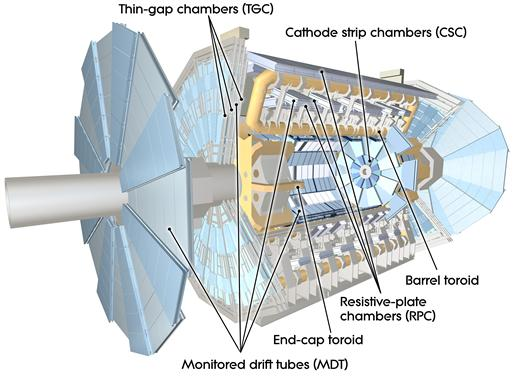
\includegraphics[width=0.8\textwidth]{figures/Detector/muons}
\captionsetup{width=0.85\textwidth} \caption{\small Schematic view of the ATLAS muon spectrometer.}
\label{sec:det:fig:ATLASMuon}
\efig

\subsubsection{Tracking chambers}

\bi
\ib \textbf{MDT} (Monitored Drift-Tube Chambers): MDTs are proportional chambers based on the drift tube technology. The tubes of 30 mm diameter are made of aluminium with a 50 $\mu$m diameter central W-Re wire. The tubes are operated with a non-flammable mixture of $93\,\%$ Ar and $7\,\%$ CO$_{2}$ at 3 bar absolute pressure; the chosen working point provides for a non-linear space-time relation with a maximum drift time of 700 ns, a small Lorentz angle, and excellent ageing properties. To improve the resolution of a chamber beyond the single-wire limit (80 $\mu$m) and to achieve adequate redundancy for pattern recognition, the MDT chambers are constructed from $2\times4$ monolayers of drift tubes for the inner station, and $2\times3$ monolayers for the middle and outer stations. The tubes are arranged in multilayer pairs of three or four monolayers, respectively, on opposite sides of a rigid support structure and placed transverse to the beam axis. A chamber provides a resolution of 40 $\mu$m, while the resolution for three layers of MDTs is 30 $\mu$m. Due to their reliability, mechanical robustness and simpler operation, MDT chambers are employed to cover the larger area of the spectrometer ($|\eta|$<2.7, 2.0 for the innermost layer).

\ib \textbf{CSC} (Cathode Strip Chambers): CSCs are multiwire proportional chambers  with cathode strip readout and with a symmetric cell in which the anode-cathode spacing is equal to the anode wire pitch. The precision coordinate is obtained by measuring the charge induced on the segmented cathode by the avalanche formed on the anode wire. The spatial resolution is $\sim40$ $\mu$m in the bending plane and $\sim$5 mm in the non-bending one. The maximum drift time for signal collection is 40 ns compared to the 700 ns of the MDTs; this gives the possibility to achieve higher acquisition rates. Due to this capability, together with the high radiation resistance, CSCs are used in the range $2.0< |\eta| <2.7$. The baseline CSC gas is a non-flammable mixture of $30\,\%$ Ar, $50\,\%$ CO$_{2}$, and $20\,\%$ CF$_{4}$; the fact that this gas contains no hydrogen  explains the low sensitivity to neutron backgrounds.
\ei


\subsubsection{Triggering chambers}

\bi

\ib\textbf{RPC} (Resistive Plate Chambers): RPCs are gaseous detectors providing a space-time resolution of 1 cm$\times$1 ns allowing single bunch-crossing discrimination. The basic RPC unit is a narrow gas gap filled with a gas mixture ($94.7\,\%$ C$_{2}$H$_{2}$F$_{4}$, $5\,\%$ Iso-C$_{4}$H$_{10}$, and $0.3\,\%$ SF$_{6}$) and formed by two parallel resistive bakelite plates.  The signal is read out via capacitive coupling by metal strips on both sides of the detector. A trigger chamber is made from two rectangular detector layers, each one read out by two orthogonal series of pick-up strips, one parallel to MDT wires and the other orthogonal to the MDT wires. RPCs provide also the $\phi$ coordinate for the tracks in the final analysis since MDTs only give the $\eta$ coordinate.

\ib\textbf{TGC} (Thin Gap Chambers): TGCs are similar to multiwire chambers with the only difference being that the anode wire pitch is larger than the cathode-anode distance. The chambers operate with a highly-quenching gas mixture of $55\,\%$ CO$_{2}$ and $45\,\%$ n-pentane (n-C$_{5}$H$_{12}$) and with wires  arranged parallel to the MDT wires provide the trigger information. They are assembled in the end-cap wheels, covering the region $1.05<|\eta|<2.7$ ($1.05<|\eta|<2.4$ for triggering). The timing resolution is comparable to the RPC's one while the spatial resolution is in the range of 2-7 mm for both coordinates.

\ei

In the barrel region, muon tracks are measured with MDT chambers and RPCs assembled on three cylindrical layers: the coordinate in the bending plane is provided by the MDT chambers, while the coordinate in the non-bending plane is provided by the RPCs (together with timing information). In the end-cap region, MDT and CSC provide the coordinate in the bending plane while the non-bending coordinate is provided by the TGCs. The muon spectrometer is designed to measure in standalone mode muons with \pt\ down to 3 $\gev$ (softer muons are stopped) and up to a few $\tev$. The momentum resolution achieved is $\sim10\%$ at $p_{T}= 1$ $\tev$. At lower energies the resolution is improved substantially by combining the track reconstructed in the muon spectrometer with a track reconstructed in the ID.
During LS1 the MS was improved targeting an increased muon acceptance. Completion of the spectrometer acceptance was already foreseen for this shutdown period, with new resistive plate chambers (RPC) placed in the barrel holes due to the toroid feet and elevators ($+2.8\%$ acceptance) and extra end-cap chambers.

\subsection{Luminosity detectors}

A good determination of the integrated luminosity is of particular importance to reach the ultimate precision in measurement of processes of interest. The luminosity in a $pp$ collider, $\lag$, defined in equation \ref{sec:det:eq:lumi}, can be expressed as well as:

\be
\lag = \frac{\mu_{\rm vis}n_{b}f_{\rm rev}}{\sigma_{\rm vis}},
\label{sec:det:eq:lumidect}
\ee

\noindent where $f_{\rm rev}$ is the collider revolution frequency, $n_{b}$ is the number of colliding bunches, and $\sigma_{\rm vis}$ is the visible inelastic cross section (total inelastic cross section times the detector acceptance and efficiency). The visible interaction rate per bunch crossing is denoted by $\mu_{\rm vis}$. It is extracted primarily from the signals coming from specific luminosity detectors. The simplest algorithm consists in simple counting of ``bunch crossings'' where detectors reported a signal, but more refined algorithms are used, in particular when the pileup contamination is no longer negligible. In order to use the measured $\mu_{\rm vis}$ for luminosity determination, each detector and algorithm must be calibrated by determining its visible cross section $\sigma_{\rm vis}$. Van der Meer scans allow to determine the effective beam size as well as the maximum achievable collision rate. These are special low-intensity LHC runs where the beam separation in the transverse planes is varied (scanned) in order to determine the beams' overlap profile.

The main detectors for luminosity measurement are listed below:
\bi

\ib \textbf{LUCID-2} (LUminosity measurements using Cherenkov Integrating Detector): It consists of 16+16 10 mm diameter Cerenkov detectors for luminosity measurements. LUCID-2 uses the thin quartz windows of photomultipliers as Cherenkov medium. To monitor the gain stability of  the photomultipliers, small sources of radioactive Bi-207 are deposited on to the quartz windows. The luminosity is measured  by not only counting hits (signals over threshold) in the detectors but also by integrating the signals. LUCID-2 is the only detector in ATLAS that can measure luminosity for individual bunches by charge integration.

\ib \textbf{BCM} (Beam Conditions Monitor): It consists of 1 cm$^{2}$ diamond detectors located at $z = 184$ cm around the beam pipe. Their fast readout and good time resolution (0.7 ps) allow them to provide luminosity information for each bunch crossing. At the same time, they are also employed to trigger on beam losses and induce the dump of the beam, thus protecting the silicon detectors from damage that might result from an uncontrolled beam.

\ib \textbf{ALFA} (Absolute Luminosity For ATLAS): It consists of eight scintillating fibers detectors placed at 240 m from the interaction point inside roman pots, above and below the beam pipe. It is a subdetector that is only activated during special runs.

\ei
In addition, cross-checks of the luminosity measurement have been performed using information from other standard subdetectors: counting of primary vertices reconstructed by the ID, and integrated signals from the Tile and forward calorimeters. The precision achieved is of a few $\%$ depending on the data-taking year.

\subsection{Trigger and data acquisition system}

Due to technical and practical limitations, not every LHC collision can be recorded by the ATLAS detector. The goal of the ATLAS trigger and data acquisition (DAQ) system is to select in real time and to record efficiently events with interesting characteristics for physics analyses. The implementation results in a multi-level system optimised to cope with the very high interaction rate and short bunch spacing of the LHC. The ATLAS trigger system is shown schematically in figure \ref{sec:det:fig:ATLASTrigger}.\par
The trigger system consists of a hardware Level 1 (L1) and a single software-based high-level trigger (HLT). This two-stage system will reduce the event rate from the bunch-crossing rate of 40 MHz to 100 kHz at L1 and to an average recording rate of 1 kHz at the HLT. During Run 1, this was a three-stage system with two stages in the HLT. In Run 2 the Event Builder and Event Filter farms are merged into a unique HLT farm for simplification and dynamic resource sharing \cite{DAQTDR}.  At L1, fast custom-made electronics find regions of interest (RoI) using the calorimeter and muon data with coarse information within a latency of 2.5 $\mu$s and keeps the information in pipeline memories. High-$\pt$ muons are identified using only the trigger chambers, RPCs in the barrel, and TGCs in the end-caps. The calorimeter selections  are  based  on  reduced-granularity  information  from  all  the  calorimeters. 
The L1 system in Run 2 consists of the L1 calorimeter trigger system (L1Calo), the L1 muon trigger system (L1Muon), new L1 topological trigger modules (L1Topo) that allow to select events on topological quantities between L1 objects within the L1 latency, and the Central Trigger Processors (CTP). 
At the HLT, fast algorithms accessing data from an RoI, or offline-like algorithms using the full-event information, run on a unique PC farm within a processing time of 0.2 s on average. At the end of 2016, a hardware track finder (FTK) is planned to be fully integrated and will provide tracks to the HLT at the L1 rates. 

\bfig[h!]
\centering
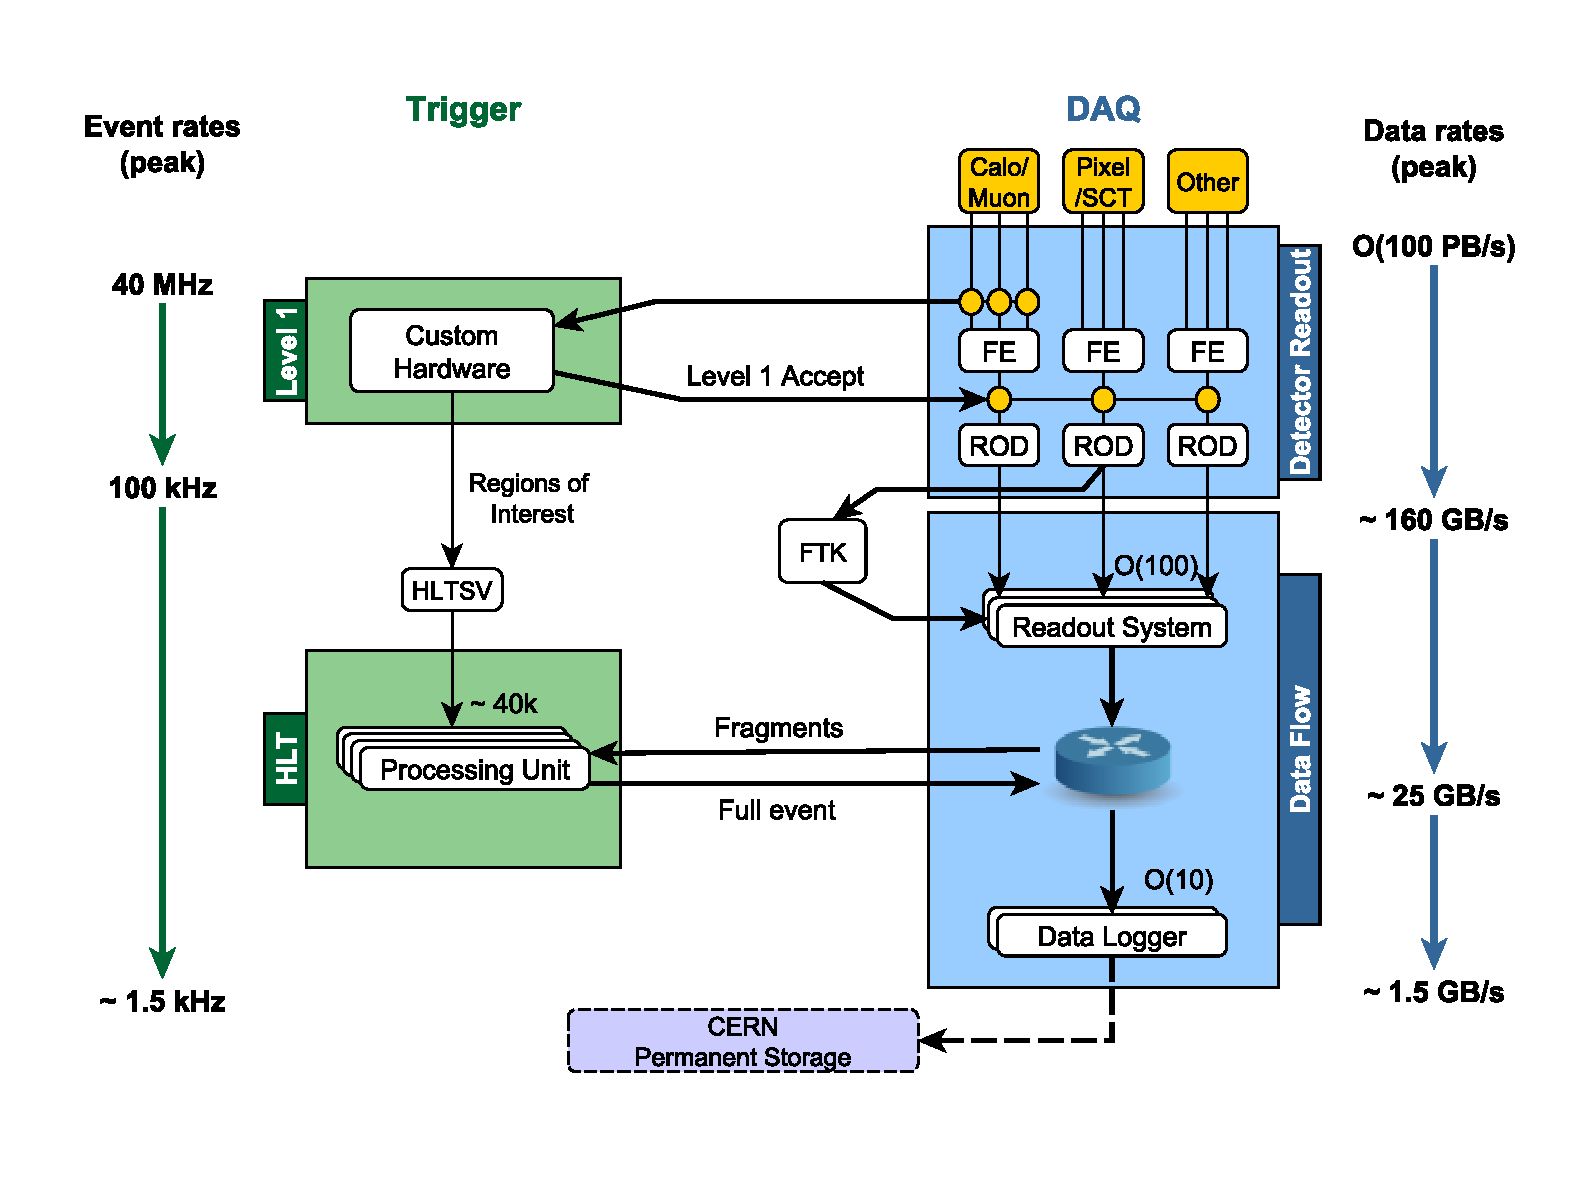
\includegraphics[width=0.82\textwidth]{figures/Detector/tdaqFullNew2016.pdf}
\captionsetup{width=0.85\textwidth} \caption{\small Schematic view of the ATLAS trigger system showing output rates in Run 2.}
\label{sec:det:fig:ATLASTrigger}
\efig


Most of the trigger chains used for physics are unscaled, meaning that all the events passing the selection are kept. Other trigger chains that contain either too many events or events considered not physically interesting are prescaled. These are characterised by a prescaling value, $P$, meaning that of all the events that activated the trigger, only 1/$P$ are accepted. These trigger chains are usually used for checks or calibration rather than physics analysis.
The term trigger chain refers to the sequence of selections that define a certain trigger object. The naming convention is:

\be
\textrm{[LEVEL][N][TYPE(S)][THRESHOLD][ISOLATION][QUALITY]},
\label{sec:det:eq:trig}
\ee


\noindent where the components, from left to right, are: the trigger level used, the multiplicity of the type, the object candidate, the threshold applied to the transverse momentum or energy of the object candidate, the object isolation, and the severity of the final algorithm requirements. Trigger chains define a trigger menu, where they are associated to their prescale value, and which is chosen based on the physics program of the data-taking period and depending on the LHC instantaneous luminosity.

\subsection{ATLAS operation}
\label{sec:det:sub:op}

The integrated luminosity for each of the two years of Run 2 is reported in figure \ref{sec:det:fig:ATLASLumi}.
The luminosity delivered by the LHC machine is shown in green while the amount of luminosity collected by the ATLAS detector is reported in yellow. The inefficiency in the data taking arises partly from the so-called ``warm start'' procedure, which consists in ramping up the voltages for the silicon detector only after the LHC has declared stable beam, or due to transient problems in the trigger and detector data acquisition. The ATLAS data-taking efficiency was above $90\%$ in both years. \par The fraction of good data delivered by each subdetector is shown in figure \ref{sec:det:fig:ATLASDQ} for both data-taking years in Run 2 so far. The fraction is $\sim90\%$ in each year; table \ref{sec:det:tab:atlum} summarises the integrated luminosity collected by ATLAS and  flagged as ``good quality data'' from all the subdetectors. For the measurements presented in this dissertation, all ATLAS subdetectors are needed, as the physics objects used in the analyses are reconstructed using the information from the full detector. The fraction of data considered was collected in the full 2015 and until July 2016, giving a total integrated luminosity of 13.2 fb$^{-1}$ at $\sqrt{s}=13$ $\tev$ satisfying data-quality requirements.

\begin{figure}[t!]
  \begin{subfigure}{0.5\textwidth}
  \centering
  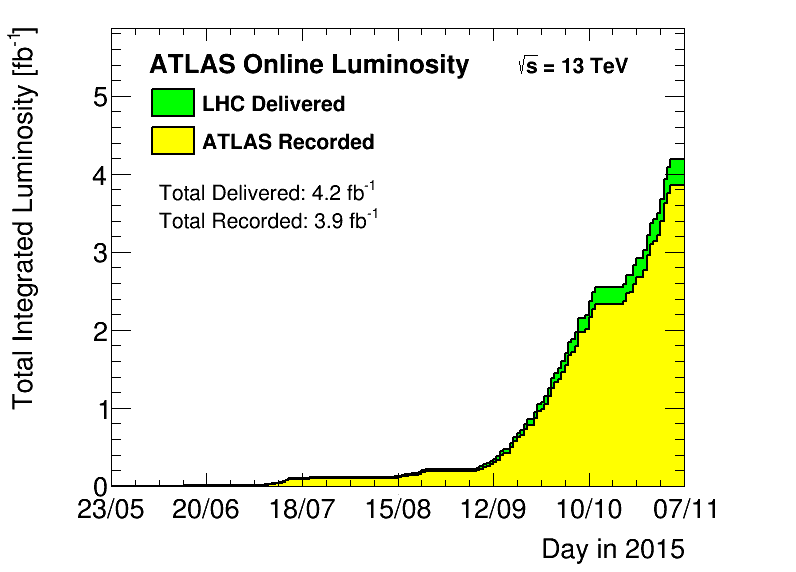
\includegraphics[width=0.9\textwidth]{figures/Detector/Lumi2015.png}
  \captionsetup{width=0.85\textwidth} \caption{\small }
  \label{sec:det:fig:lumi15}
\end{subfigure}
\begin{subfigure}{0.5\textwidth}
  \centering
  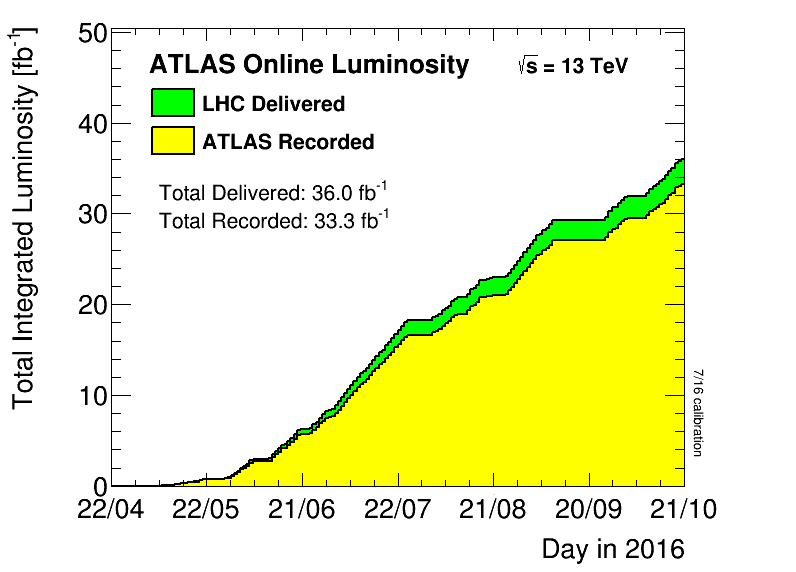
\includegraphics[width=0.9\textwidth]{figures/Detector/Lumi2016.png}
  \captionsetup{width=0.85\textwidth} \caption{\small }
  \label{sec:det:fig:lumi16}
\end{subfigure}

\captionsetup{width=0.85\textwidth} \caption{\small Integrated luminosity delivered by the LHC in the years (a) 2015 and (b) 2016 as a function of time. Also shown is the integrated luminosity recorded by ATLAS.}
\label{sec:det:fig:ATLASLumi}
\end{figure}


\bfig[b!]
\centering
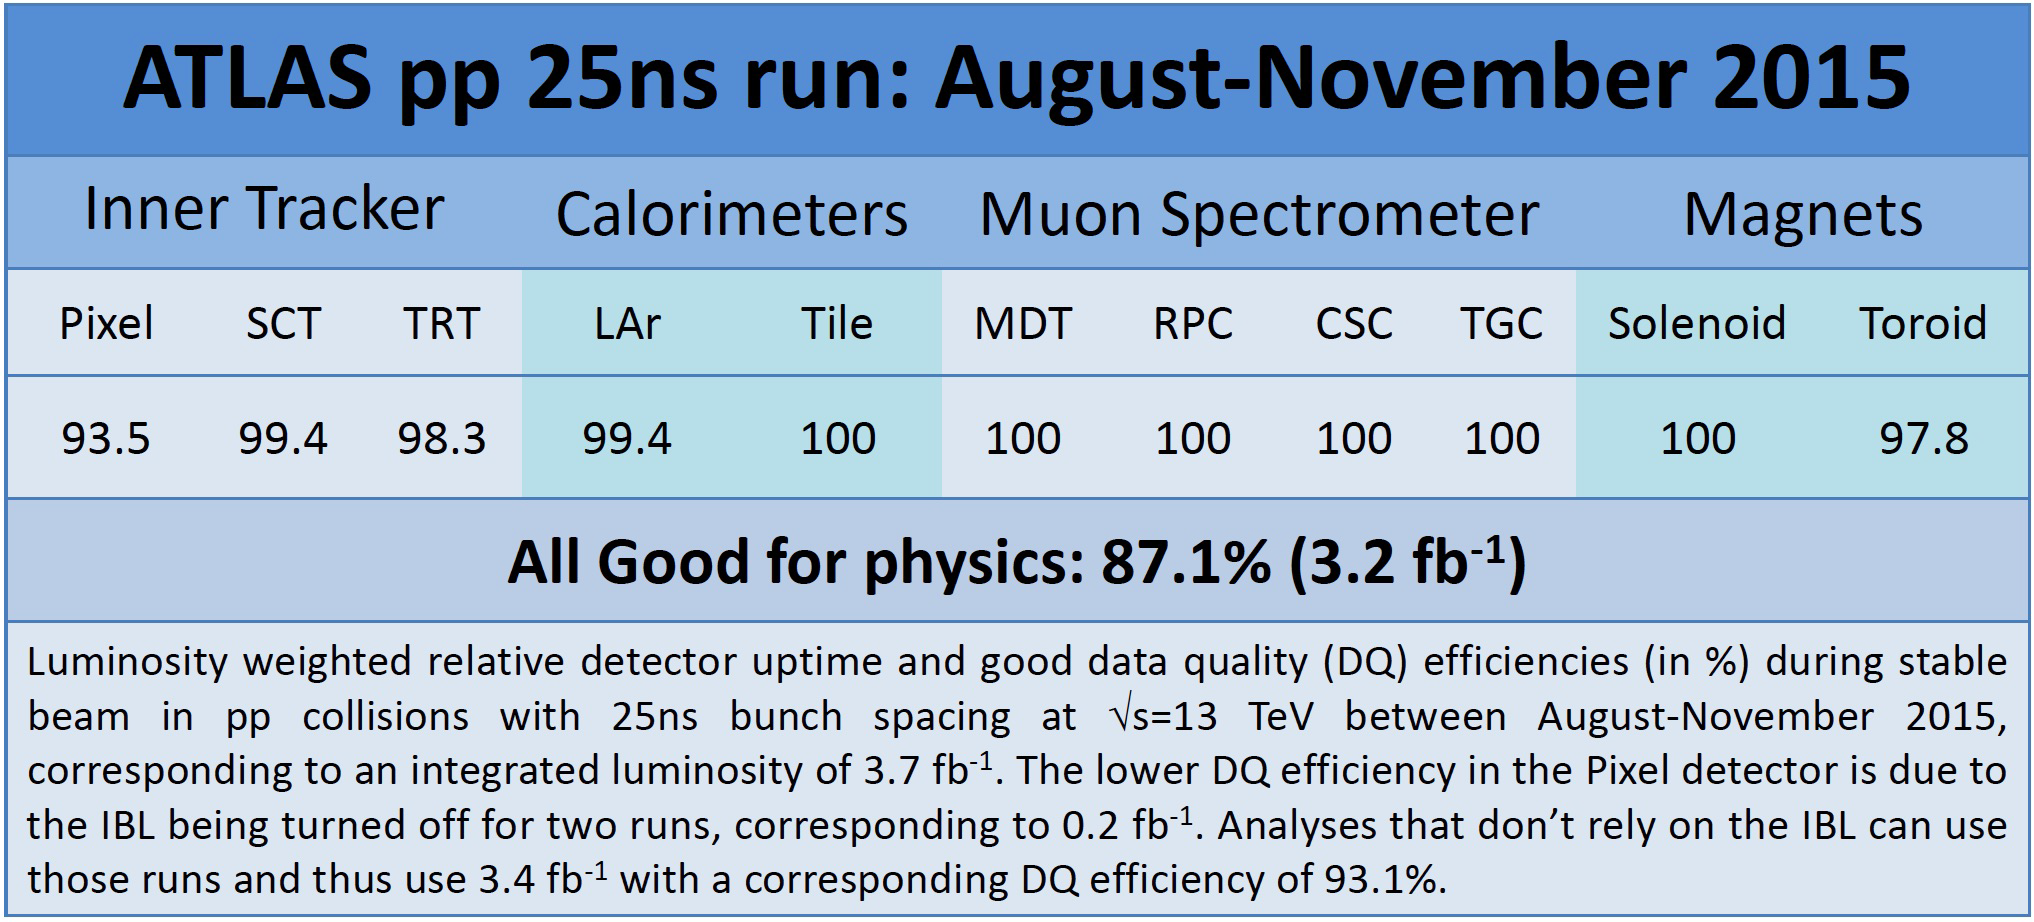
\includegraphics[width=0.85\textwidth]{figures/Detector/DQ2015.png}
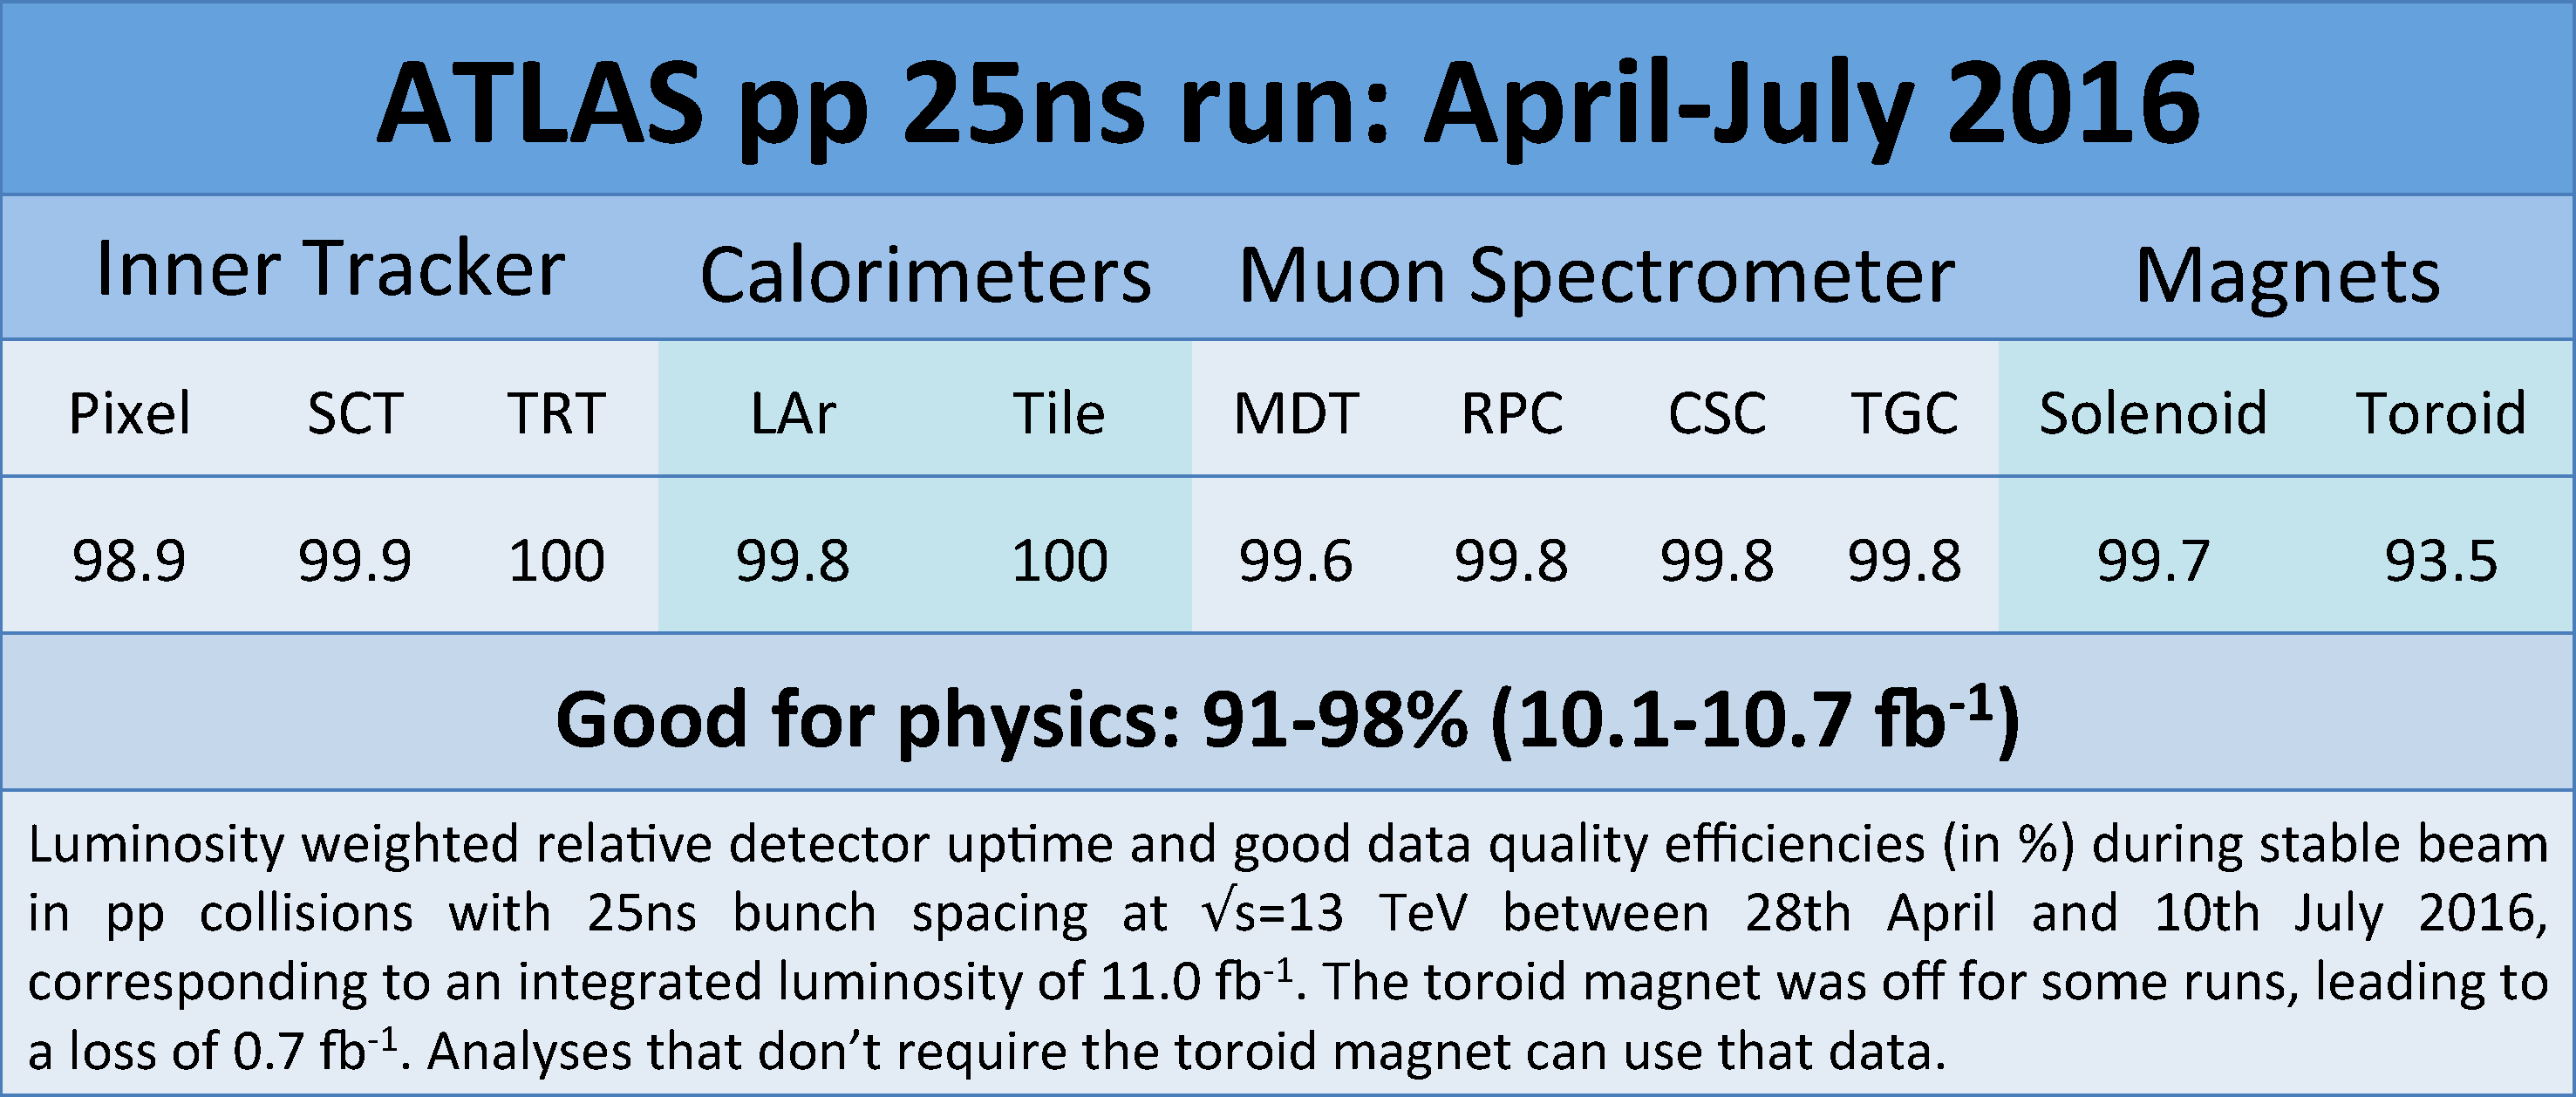
\includegraphics[width=0.85\textwidth]{figures/Detector/DQ2016.png}
\captionsetup{width=0.85\textwidth} \caption{\small Fraction of good data delivered by each subdetector during the year 2015 (top) and 2016 (bottom).}
\label{sec:det:fig:ATLASDQ}
\efig



\begin{table}
\begin{center}
\begin{tabular}{c|c|c|c}
  \hline \hline
  year & LHC delivered & ATLAS recorded & ATLAS good quality \\
  \hline
 2015 & 4.2 fb$^{-1}$ & 3.9 fb$^{-1}$ & 3.2 fb$^{-1}$ \\
 2016 & 38.9 fb$^{-1}$ & 35.9 fb$^{-1}$ & 33.2 fb$^{-1}$ \\
  
  \hline\hline

\end{tabular}
\captionsetup{width=0.85\textwidth} \caption{\small Integrated luminosity per year during Run 2. Columns correspond to LHC delivered luminosity, luminosity recorded by ATLAS, and luminosity with good data quality flag from all subdetectors.}
\label{sec:det:tab:atlum}
\end{center}
\end{table}



\subsection{Future ATLAS upgrades}

In the next years, the LHC will undergo a  series  of  upgrades  leading  ultimately  to  a five-fold  increase  of  the  instantaneous  luminosity  with  leveling according to the High-Luminosity LHC (HL-LHC) project \cite{BejarAlonso:2069130}.  The goal is to extend the dataset from about 300 fb$^{-1}$, expected to be collected by the end of the LHC run (in 2022), to 3000 fb$^{-1}$ by 2035. The foreseen higher  luminosity  at  the  HL-LHC  represents  a  great  challenge  for  ATLAS.\par
A  second  shutdown  (LS2)  is  being  planned  in  2018  to  integrate  the  Linac4  into  the  injector  complex,  to increase the energy of the PS Booster, to reduce the beam emittance, and to upgrade the collider collimation system.  When data taking resumes in 2020, the peak luminosity is expected to reach $\sim 2-3 \times 10^{34}$ cm$^{-2}$s$^{-1}$, corresponding  to  55  to  80  interactions  per  crossing  with  25  ns  bunch  spacing,  well  beyond  the initial  design  goals.
Therefore, to  face the increased event rates, ATLAS will undergo to several upgrades during this long shutdown, referred to as Phase-I upgrade:
\bi
\ib A  replacement  of  the   first  endcap  station  of the  MS,  the  New  Small  Wheel  (NSW) \cite{NSW},  is  proposed.   The  NSW  must  ensure  efficient tracking at high particle rate (up to $5 \times 10^{30}$ cm$^{-2}$s$^{-1}$) and larger $|\eta|$, with position resolution of $<100$ $\mu$m. Furthermore, unlike the present layer, the NSW will be integrated into the Level-1 trigger, thus helping in rejecting background by selecting tracks coming from the primary interaction and matched with the most external layers of the muon spectrometer.
\ib The calorimeter trigger \cite{CALORUP} will also have a an upgrade in Phase I, with the goal of providing higher-granularity,  higher-resolution and longitudinal shower information from the calorimeter to the Level-1 trigger processors.
\ib The Fast TracKer (FTK) \cite{FTK} Trigger will perform the track  finding and  fitting on-line using dedicated massive parallel processing.  FTK will then provide the track parameters with resolution close to that of offline tracks shortly after the start of the Level-2 processing, thus releasing extra resources for more advanced selection algorithms, which ultimately could improve the performance of tracking-based  filter algorithms such as $b$-tagging and $\tau$ identification. While the full geometrical coverage for full Phase-I pileup in foreseen after the 2018 shutdown, a progressive coverage and commissioning already started in 2015.\\
\ei
\noindent The  Phase-I  upgrades  are  designed  to  be  fully  forward-compatible  with  the  physics  programme  of  the  high luminosity HL-LHC (Phase II), when the instantaneous luminosity should reach $\sim 5-7 \times 10^{34}$ cm$^{-2}$ s$^{-1}$, giving 200 interactions per crossing and a total integrated luminosity of 3000 fb$^{-1}$.\par
A third 36-months long shutdown (LS3) in 2023-25 will be necessary to upgrade the accelerator to this ultimate operation mode. ATLAS is being planning major updates in all its subsystems and trigger architecture. The present ATLAS Inner tracker will have several limitations in Phase II, when up to 200 pileup events per bunch crossing are expected.  The entire Inner Detector will be replaced with a new, all-silicon Inner Tracker (ITk) \cite{ITK} with pixel sensors at the inner radii surrounded by microstrip sensors.  A new trigger architecture is being developed that is compatible with the constraints imposed by the detector and provides a  flexible trigger with the potential to deliver the required performance. As currently envisaged, the baseline design for the Phase-II Trigger foresees a split Level-0/Level-1 hardware trigger with a total L1 accept rate of 200 kHz and total latency of 20 $\mu s$.





